\subsection{External Interface Requirements}
\subsubsection{User Interfaces}
The images below show the most important screens of the application.
\begin{figure}[H]
\centering
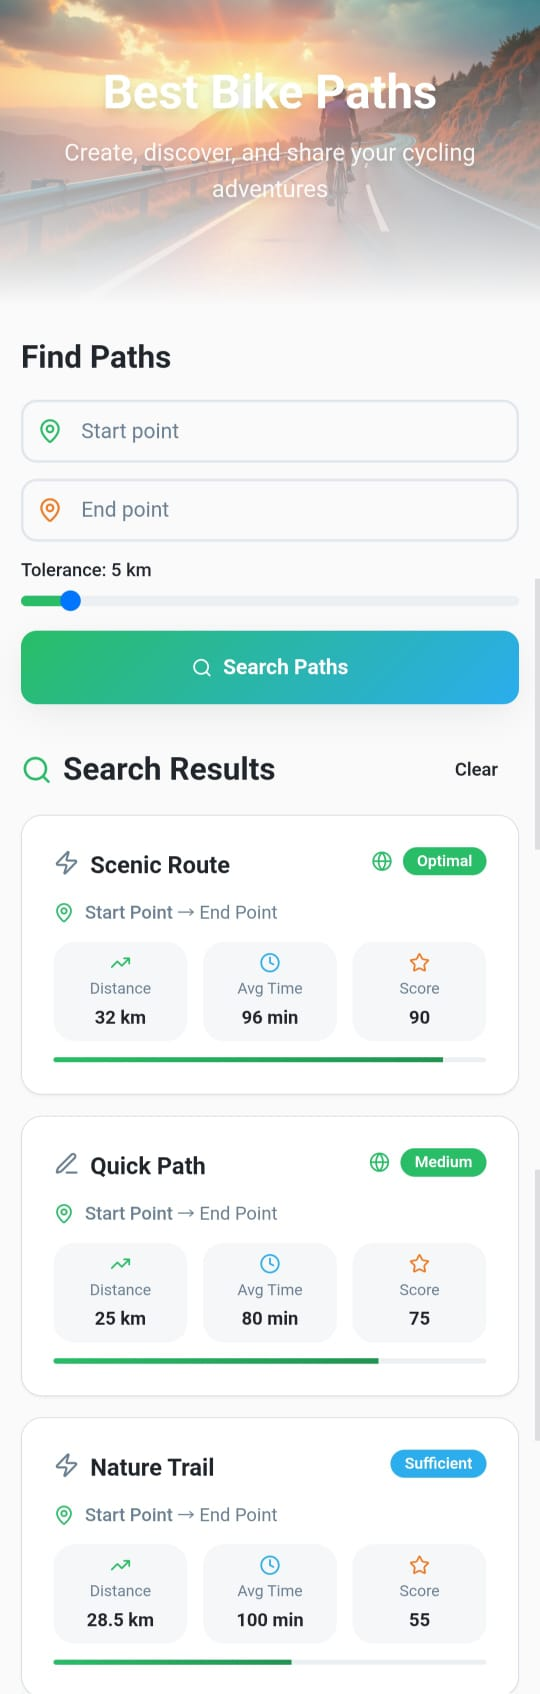
\includegraphics[width=0.4\linewidth]{Images/User Interface/Search1.jpeg}
\hspace{1.3cm}
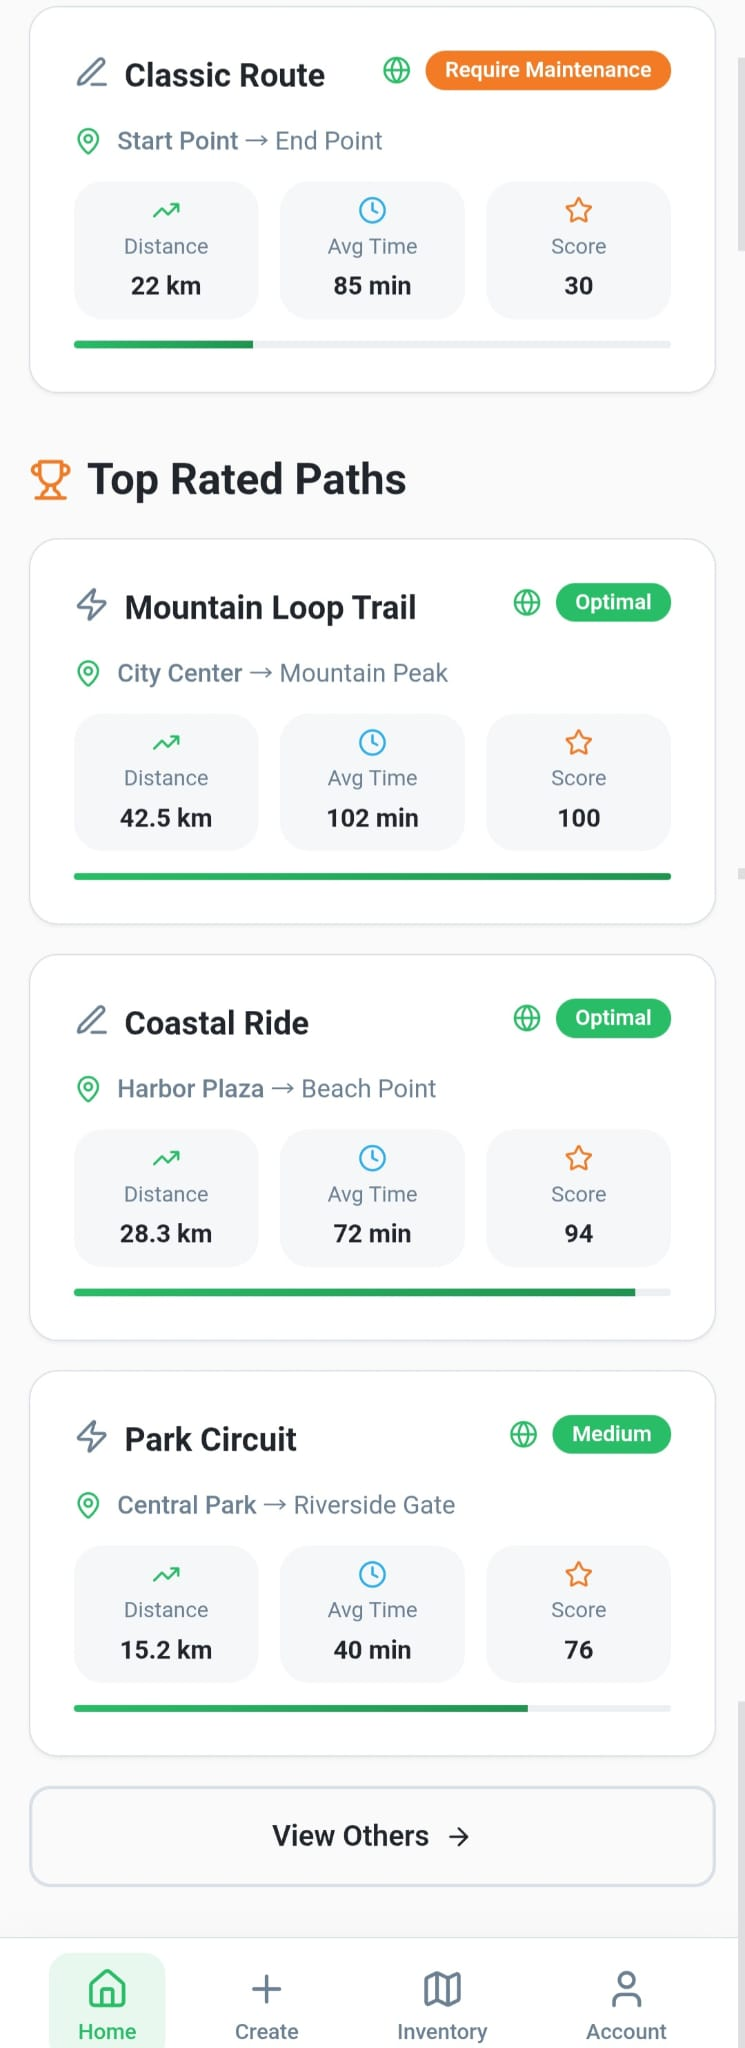
\includegraphics[width=0.4\linewidth]{Images/User Interface/Search2.jpeg}
\caption{Screens of \textit{Homepage}}
\label{fig:Homepage}
\end{figure}
\begin{figure}[H]
\centering
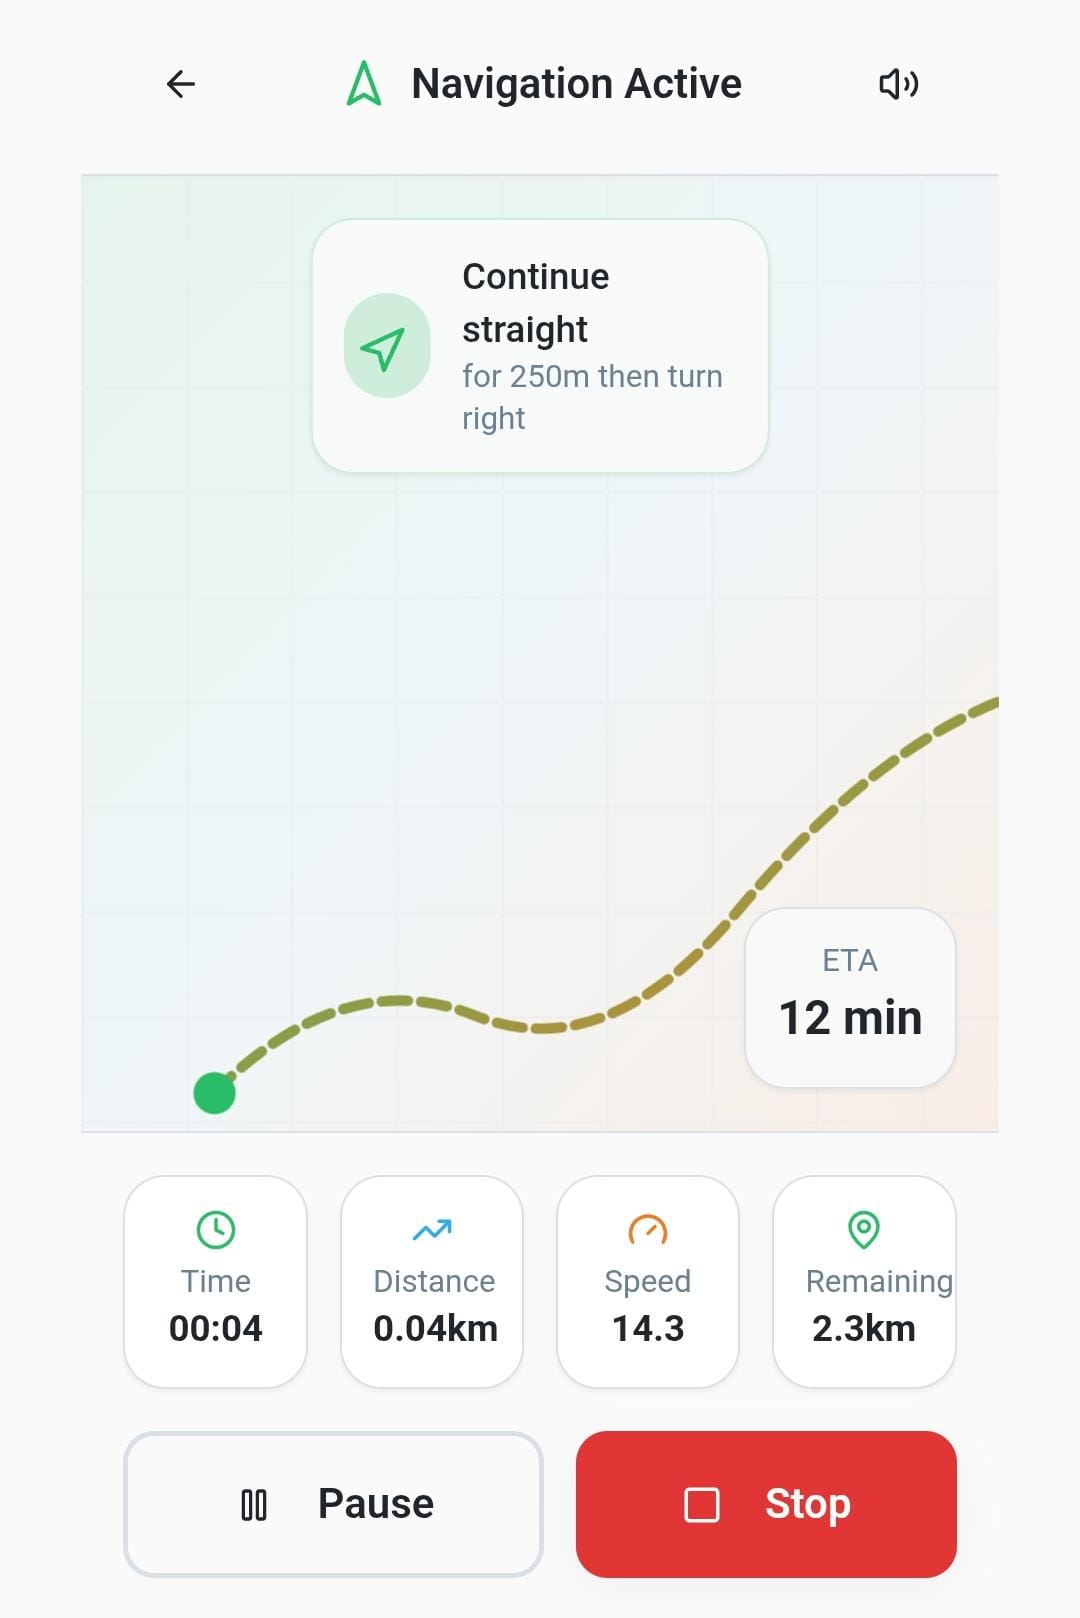
\includegraphics[width=0.4\textwidth]{Images/User Interface/Navigation.jpeg}
\caption{Screen of \textit{Navigation}}
\label{fig:Navigation}
\end{figure}
\begin{figure}[H]
\centering
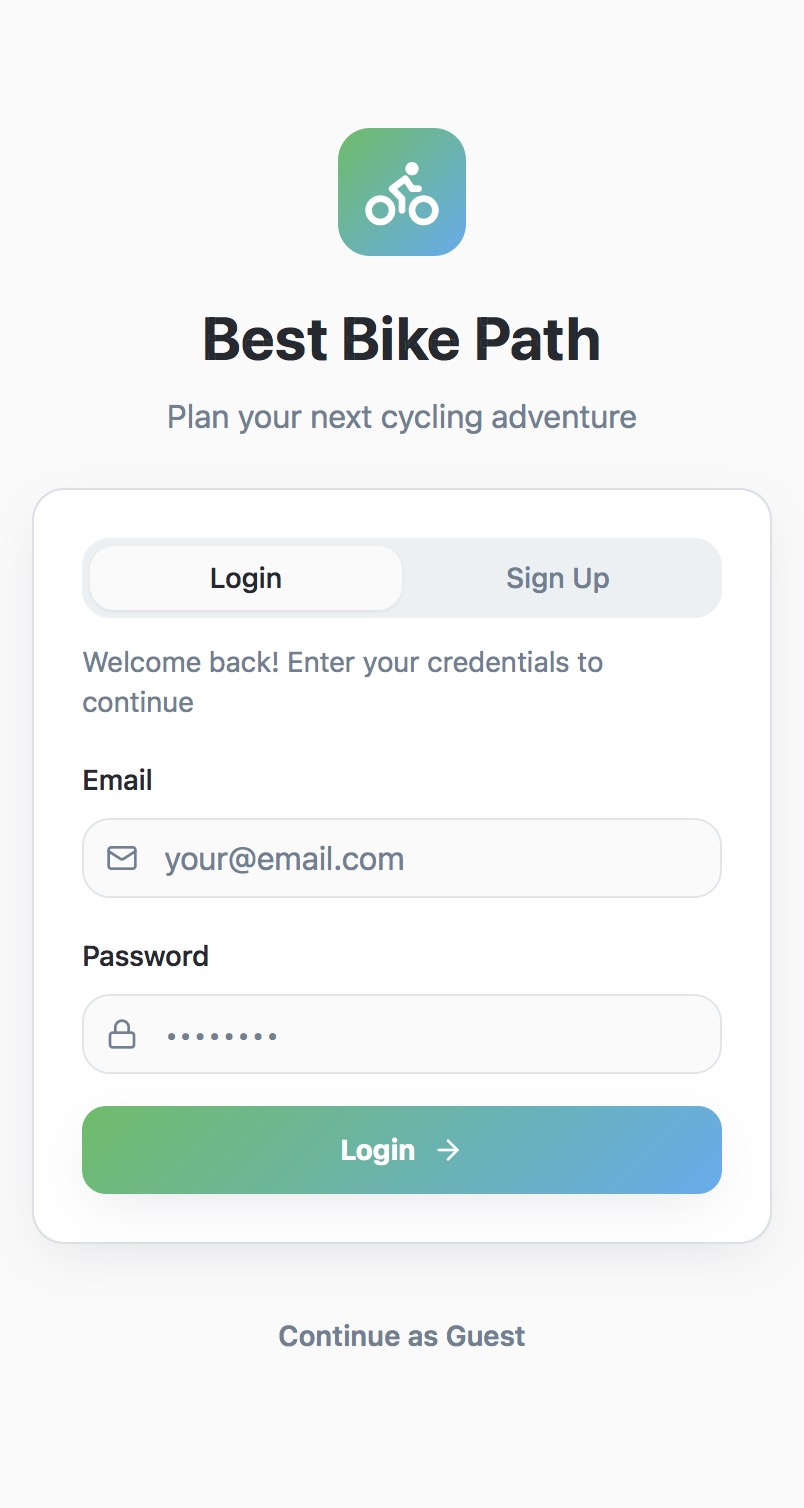
\includegraphics[width=0.4\textwidth]{Images/User Interface/SignUp.JPG}
\hspace{1.3cm}
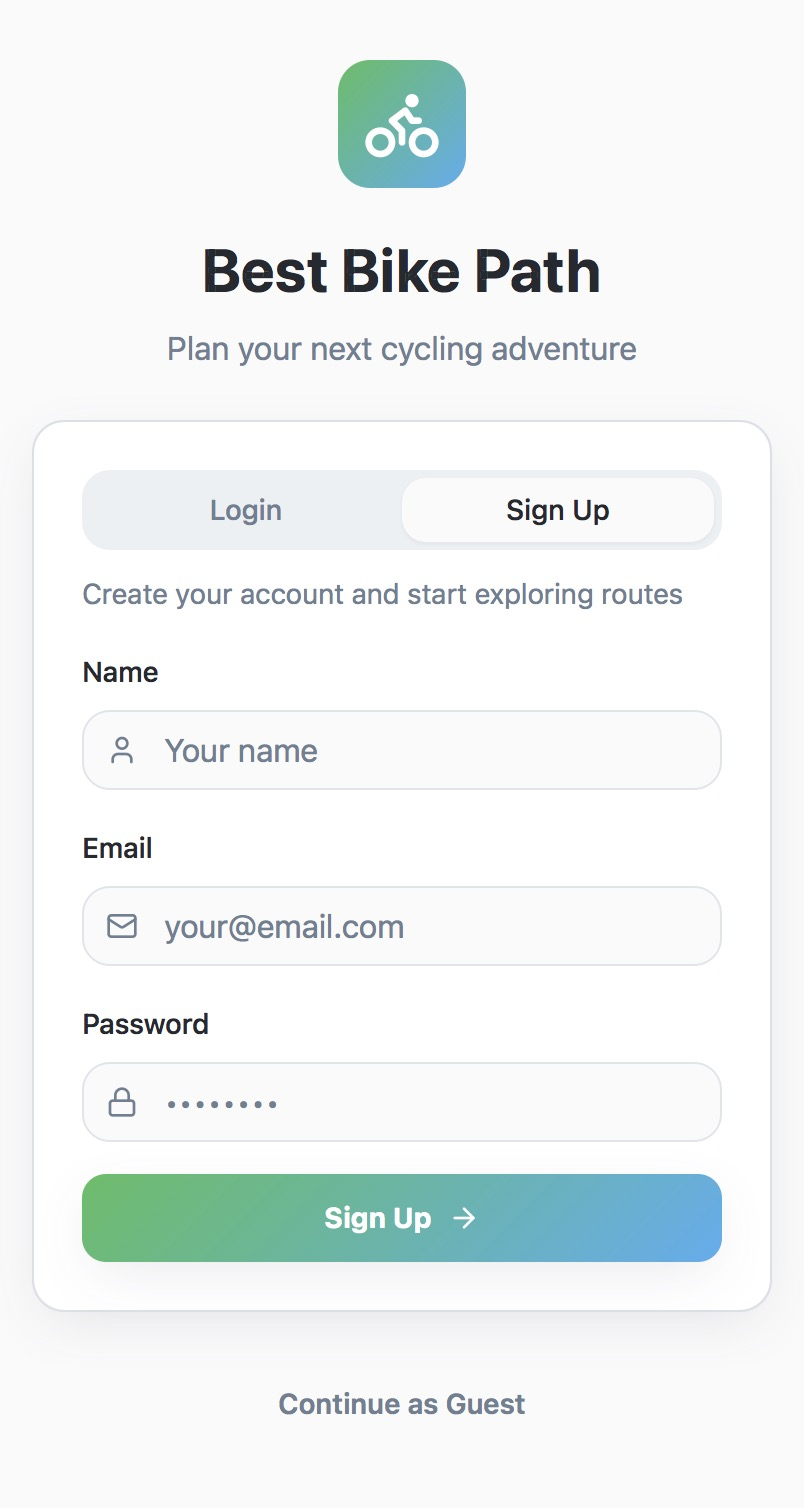
\includegraphics[width=0.4\textwidth]{Images/User Interface/Login.JPG}
\caption{Screens of  the Authentication pages: \textit{Login} and \textit{SignUp}}
\label{fig:LoginSignUp}
\end{figure}
\begin{figure}[H]
\centering
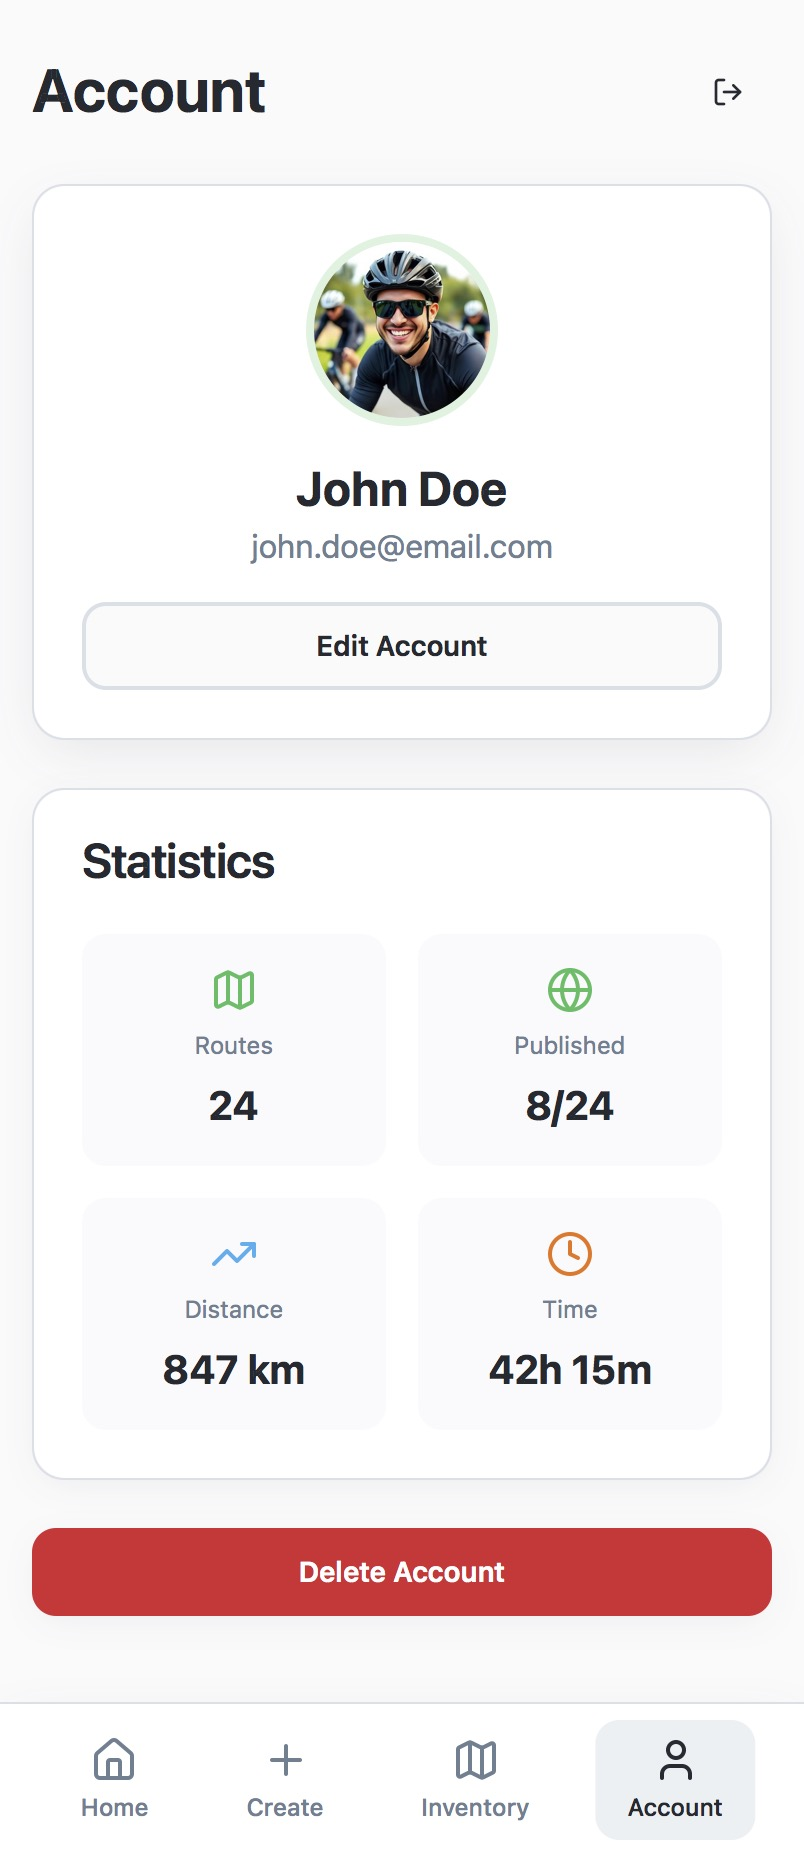
\includegraphics[width=0.4\textwidth]{Images/User Interface/Account.JPG}
\hspace{1.3cm}
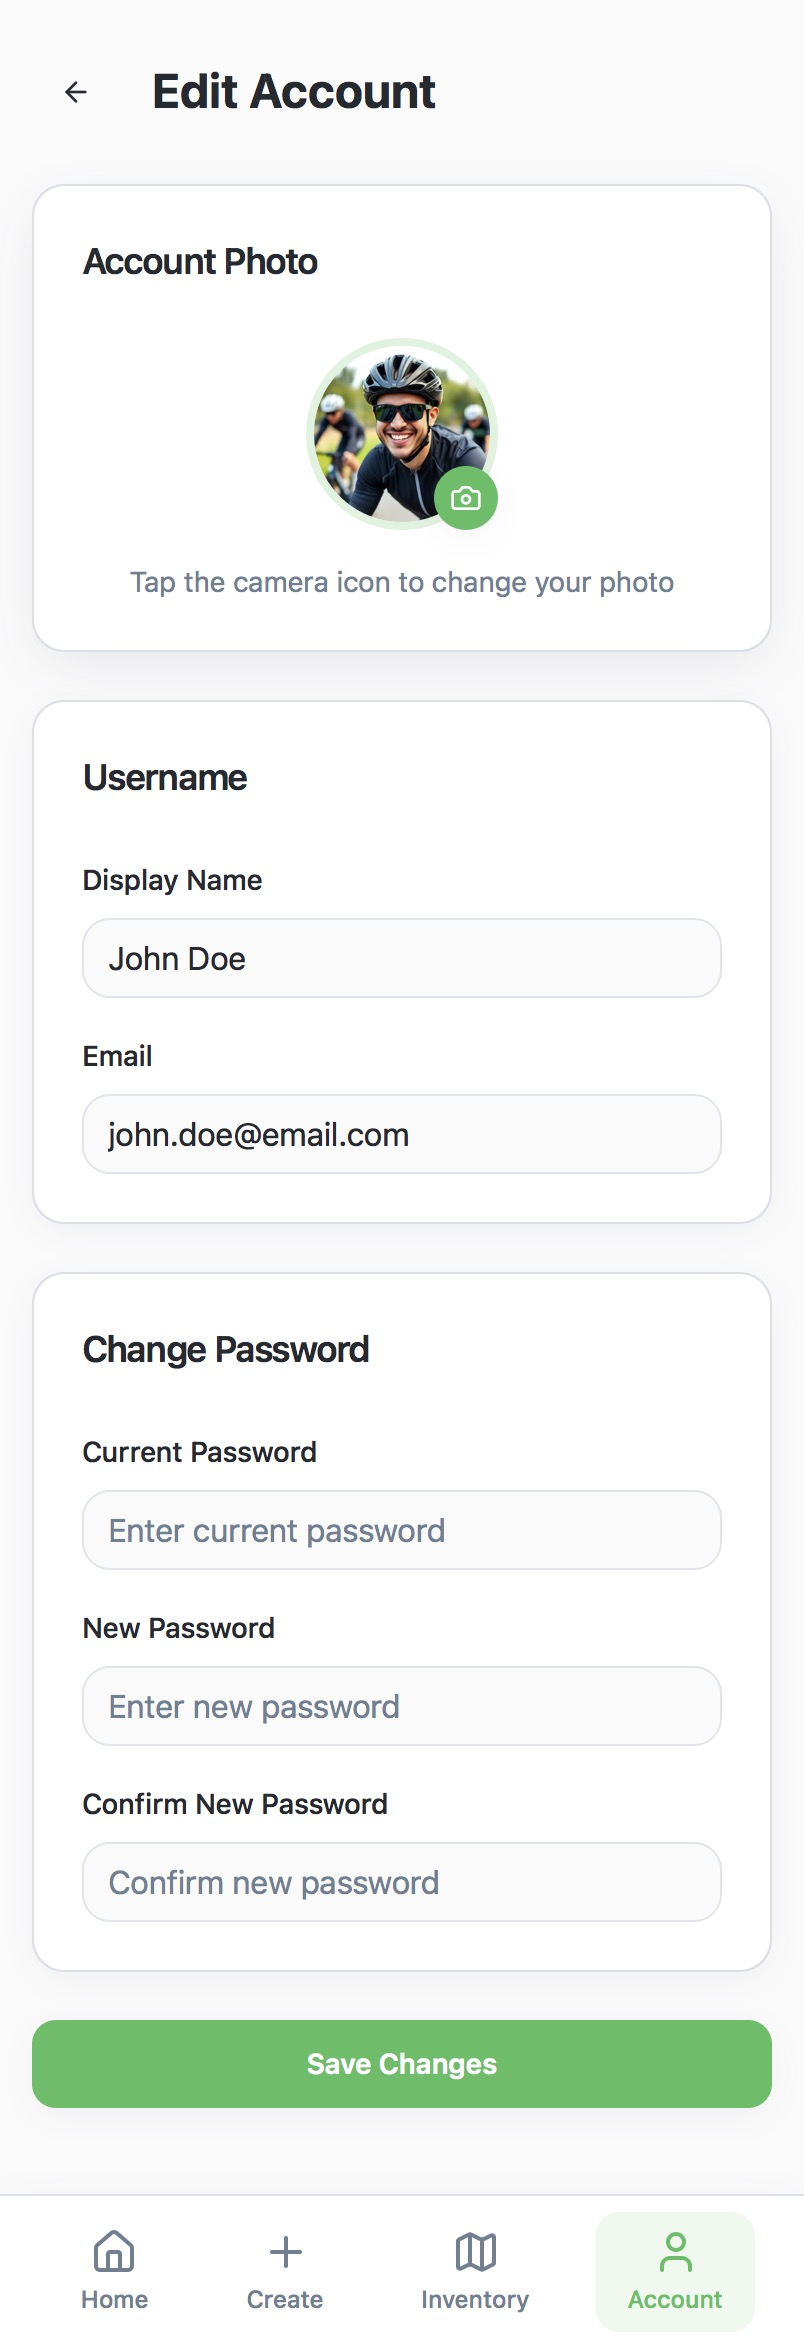
\includegraphics[width=0.4\textwidth]{Images/User Interface/EditAccount.JPG}
\caption{Screens of \textit{Account} and \textit{Edit Account}}
\label{fig:Account}
\end{figure}
\begin{figure}[H]
\centering
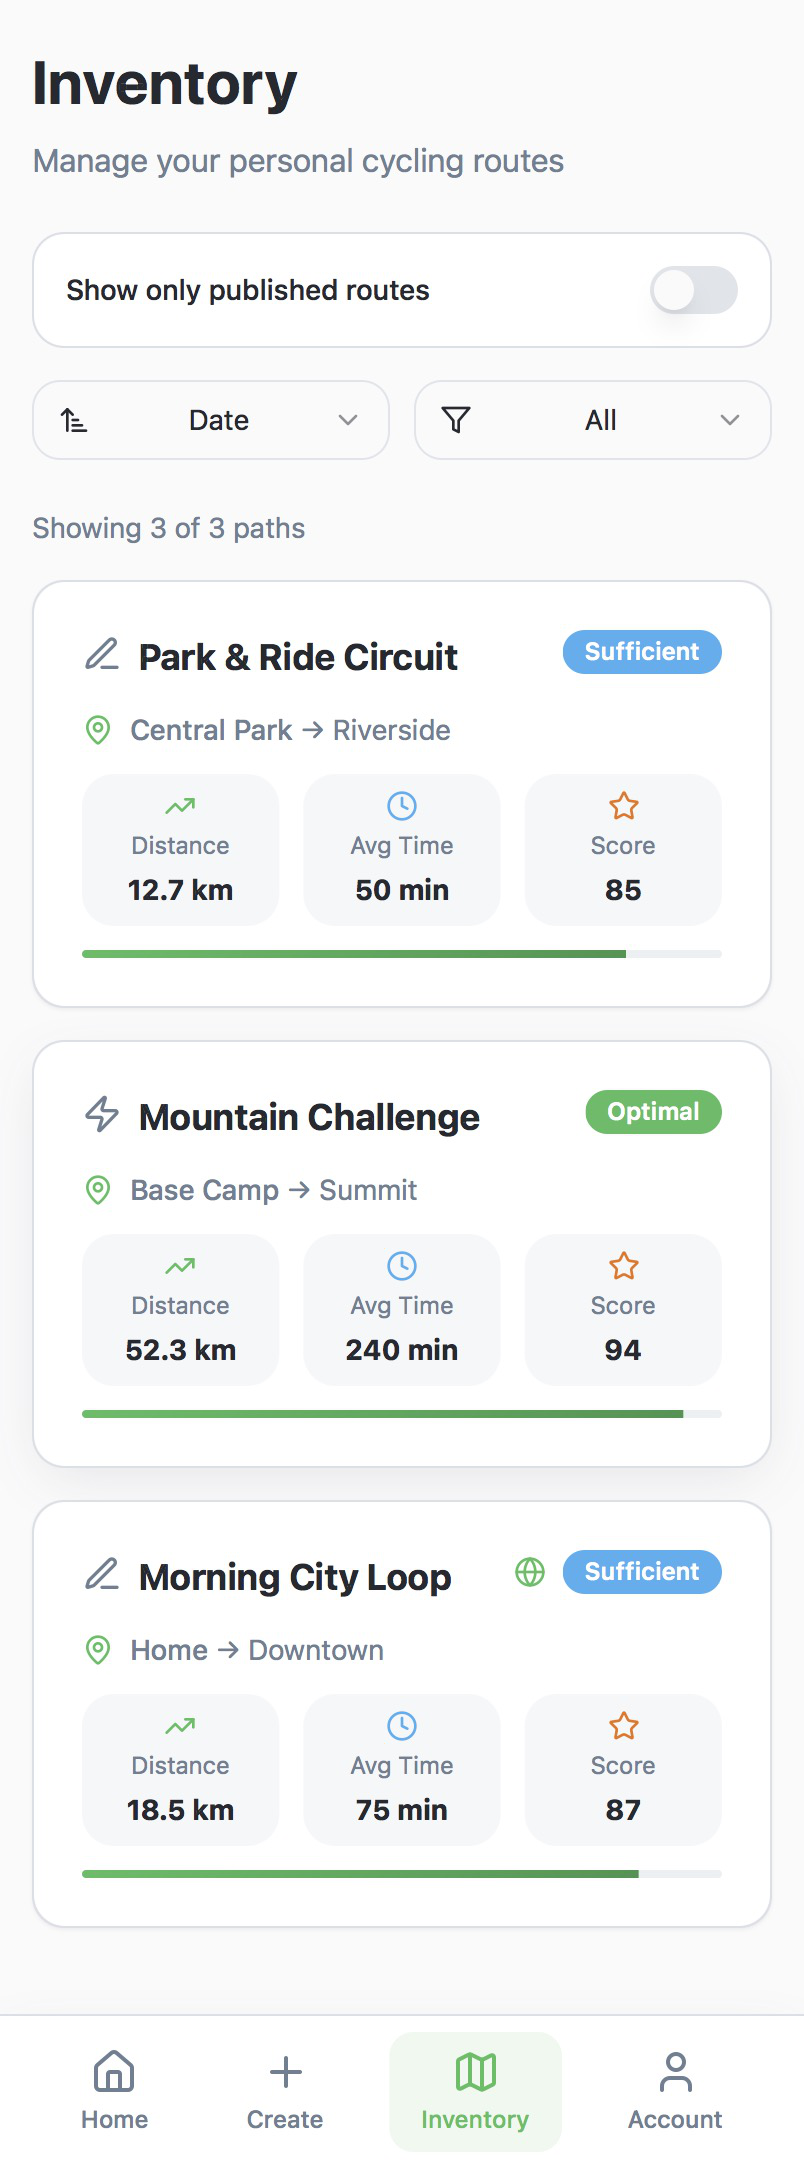
\includegraphics[width=0.4\textwidth]{Images/User Interface/inventory.png}
\hspace{1.3cm}
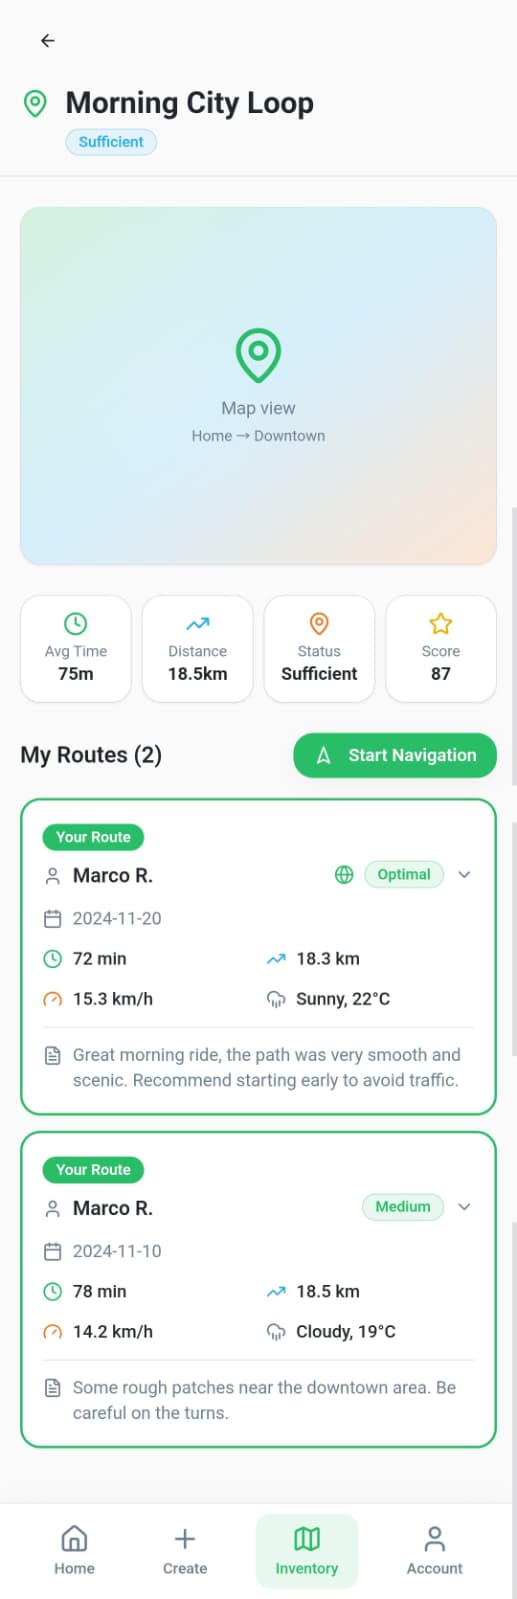
\includegraphics[width=0.4\textwidth]{Images/User Interface/MyRoute.jpeg}
\caption{Screens of \textit{Inventory} and \textit{Path's details}}
\label{fig: page to add route’s details}
\end{figure}
\begin{figure}[H]
\centering
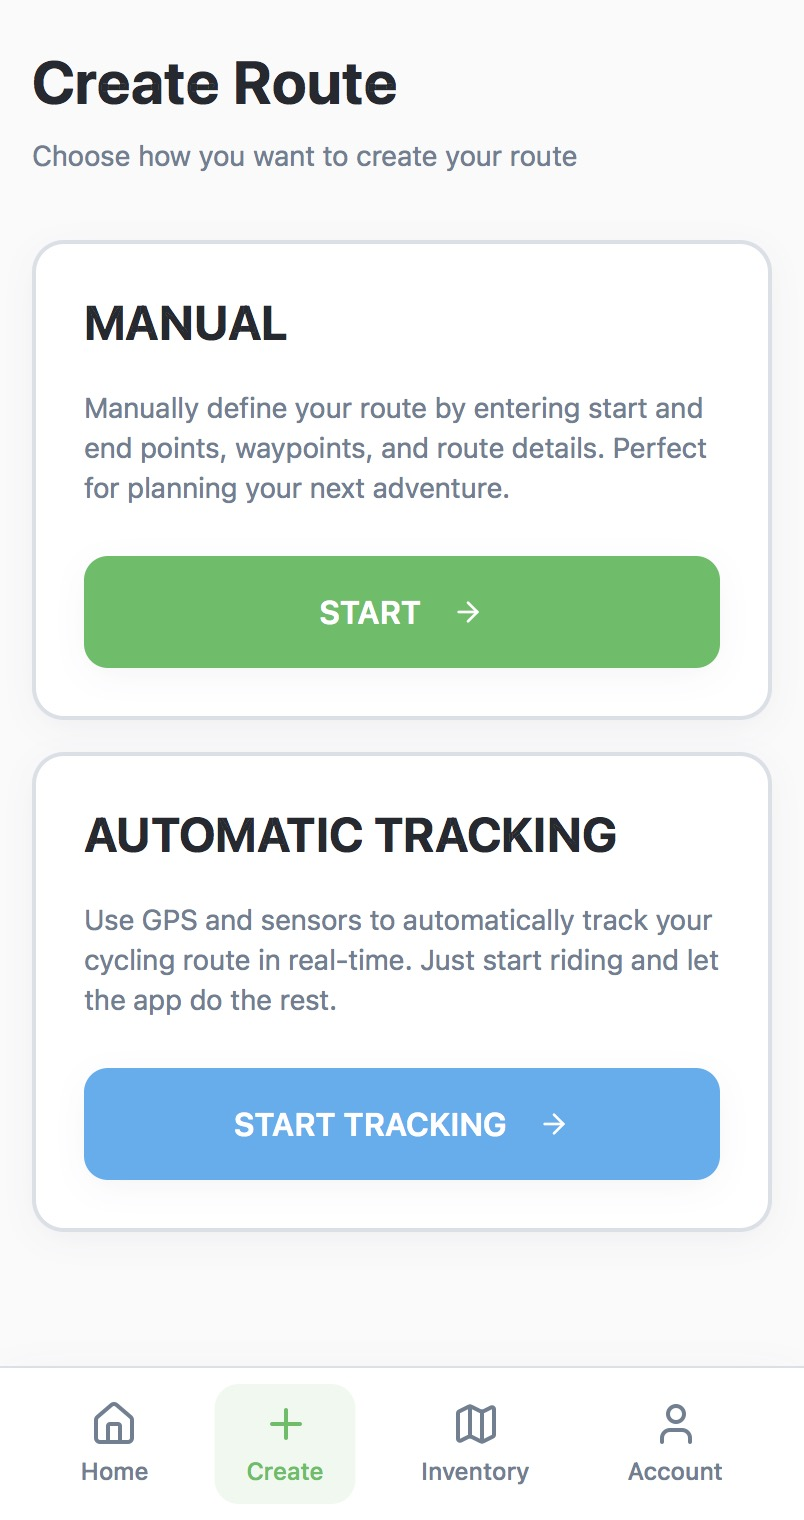
\includegraphics[width=0.34\textwidth]{Images/User Interface/CreateRoute.JPG}
\hspace{1.3cm}
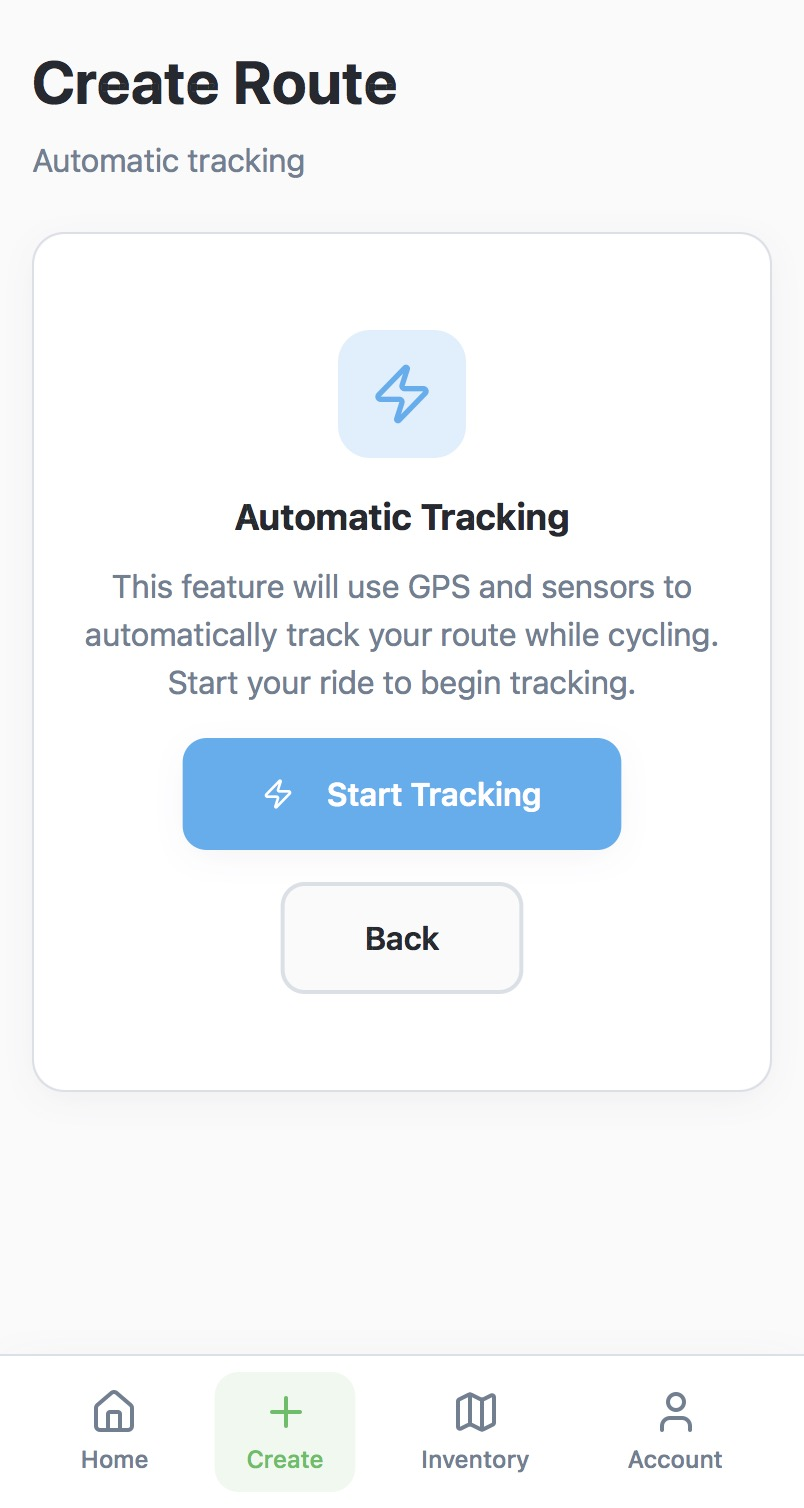
\includegraphics[width=0.34\textwidth]{Images/User Interface/AM.JPG}
\caption{Screens of \textit{Create Route} and \textit{Create Route (Automatic Mode)}}
\label{fig:CreateRoute}
\end{figure}
\begin{figure}[H]
\centering
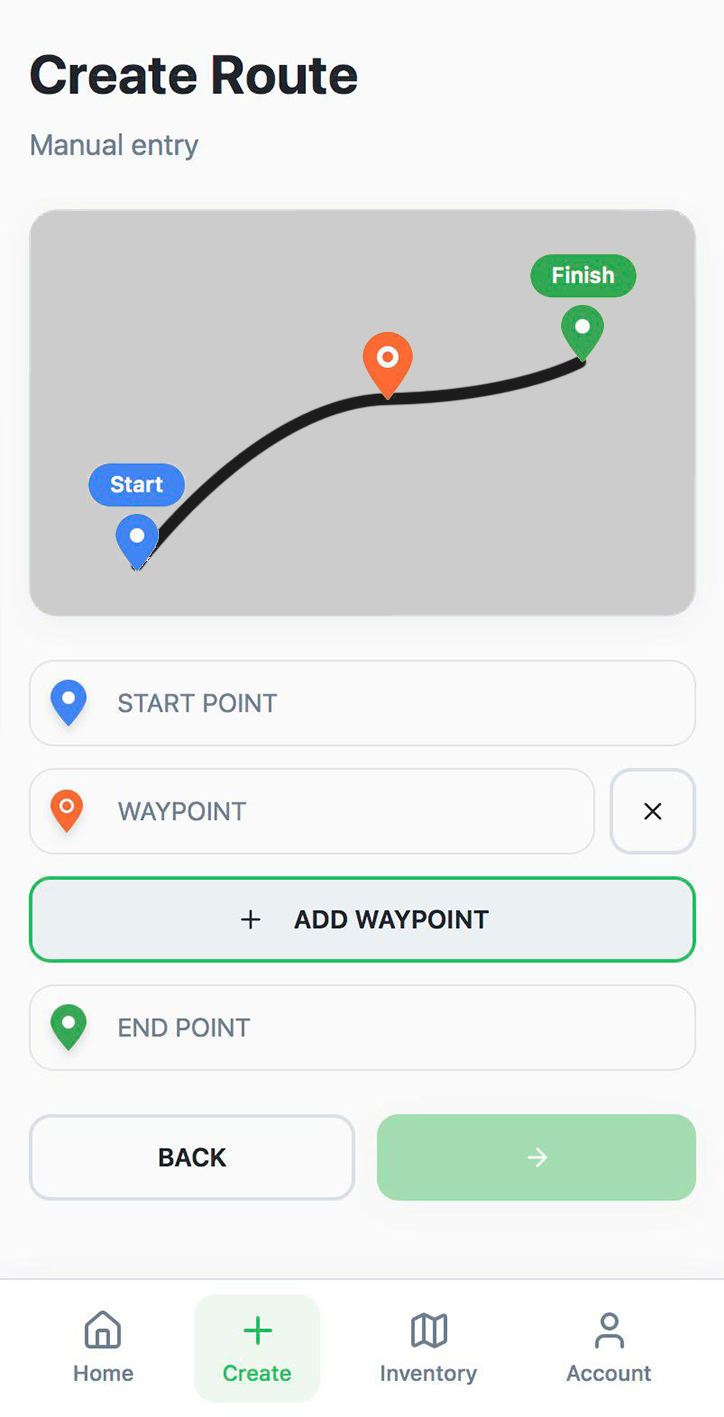
\includegraphics[width=0.34\textwidth]{Images/User Interface/MM.JPG}
\hspace{1.3cm}
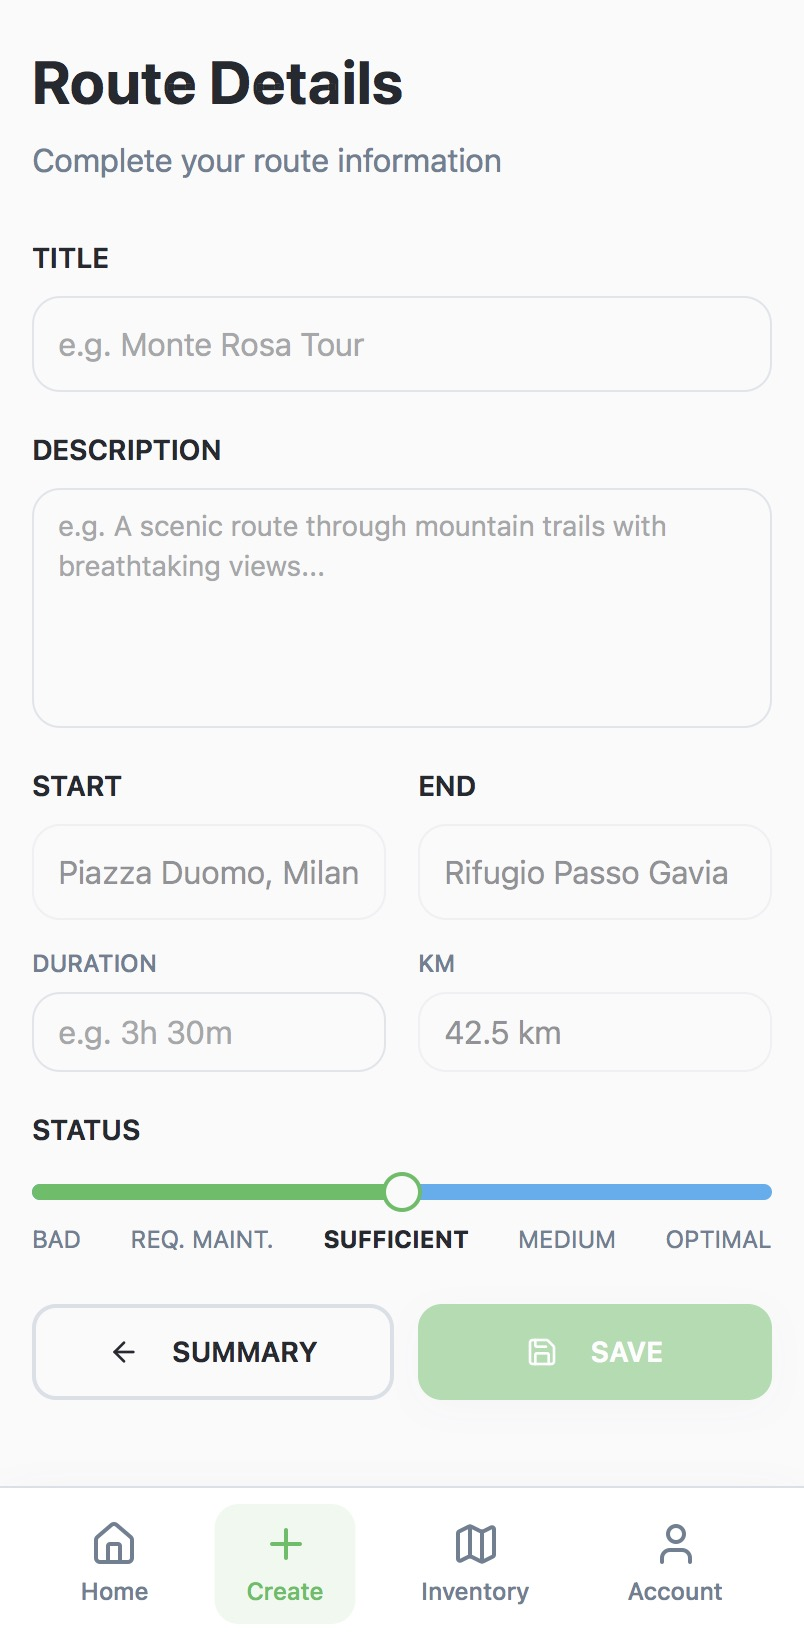
\includegraphics[width=0.34\textwidth]{Images/User Interface/Details.JPG}
\caption{Screens of \textit{Create Route (Manual Mode)} and \textit{Route Details}}
\label{fig:CreateRouteManualDetails}
\end{figure}
\subsubsection{Hardware Interfaces} 
The platform is designed to be used on mobile devices taking advantage of their sensors.\\
The system interacts with several hardware components to provide its functionality, especially for the automatic path acquisition. In particular, the system uses the GPS sensor to track the cyclist's position in real time, while the accelerometer and gyroscope are used to detect and analyze the characteristics of the path.
\subsubsection{Software Interfaces}
The system implements a mapping solution based on pre-existing tools such as \textit{OpenStreetMap} and its associated features. This allows users to create and visualize paths and to follow them using the navigation system.  
\subsubsection{Communication Interfaces}
Cyclists use the Internet to access to the platform. An Internet connection is strictly required when users search for a path or publish a route as well as when the system indirectly communicates with the weather service to retrieve meteorological information to enrich a route before saving it. \\
To prevent data breaches, the software must protect exchanged data and avoid exposing sensitive information, such as the location of a user in real time or the credentials. To achieve this, communications must be secured using HTTPS to encrypt data during transmission. 
\subsection{Functional Requirements}
\textbf{Sign-up e Login}
\begin{itemize}
    \item \textbf{R1:} The platform allows the Cyclists to create an account.
    \item \textbf{R2:} The platform allows Cyclists to authenticate.
    \item \textbf{R3:} The platform allows the access as a Guest. 
    \item \textbf{R4:} The platform allows Cyclists to view their personal account.
    \item \textbf{R5:} The platform allows Cyclists to modify their personal account.
\end{itemize}
\textbf{Route Creation and Publication}
\begin{itemize}
    \item \textbf{R6:} The platform allows the Cyclists to create a new route through a manual creation process.
    \item \textbf{R7:} The platform allows the Cyclists to create a new route through an automatic creation process.
    \item \textbf{R8:} The platform allows the Cyclists to confirm and complete the automatically acquired information.
    \item \textbf{R9:} The platform collects data from the device sensors.
    \item \textbf{R10:} The platform collects weather data and enriches the path's statistics.
    \item \textbf{R11:} The platform allows the Cyclists to evaluate the status of a route. 
    \item \textbf{R12:} The platform allows the Cyclists to publish/unpublish a route.
    \item \textbf{R13:} The platform allows the Cyclists to delete a route.
\end{itemize}
\bigskip\bigskip
\textbf{Route Visualization}
\begin{itemize}
    \item \textbf{R14:} The platform allows the Cyclists to visualize a list of paths in the personal inventory with the possibility to filter them.
    \item \textbf{R15:} The platform allows the User to view the details of a path such as the map, the statistics and the status.
    \item \textbf{R16:} The platform allows the User to visualize the details of the routes related to a path.
\end{itemize}
\textbf{Route Search and Navigation}
\begin{itemize}
    \item \textbf{R17:} The platform allows the User to search a path by setting the start and the end points with a kilometer tolerance.
    \item \textbf{R18:} The platform suggests to the User a list of available routes ranked by score.
    \item \textbf{R19:} The platform supports path navigation by allowing users to follow routes that have been previously created.
\end{itemize}
\textbf{Scoring, Merging and Ranking}
\begin{itemize}
    \item \textbf{R20:} The platform merges the status when more than one is present.
    \item \textbf{R21:} The platform computes a score for each path based on path's status and average speed.
\end{itemize}
\subsubsection{Use Case Diagram}
\begin{figure}[H]
\centering
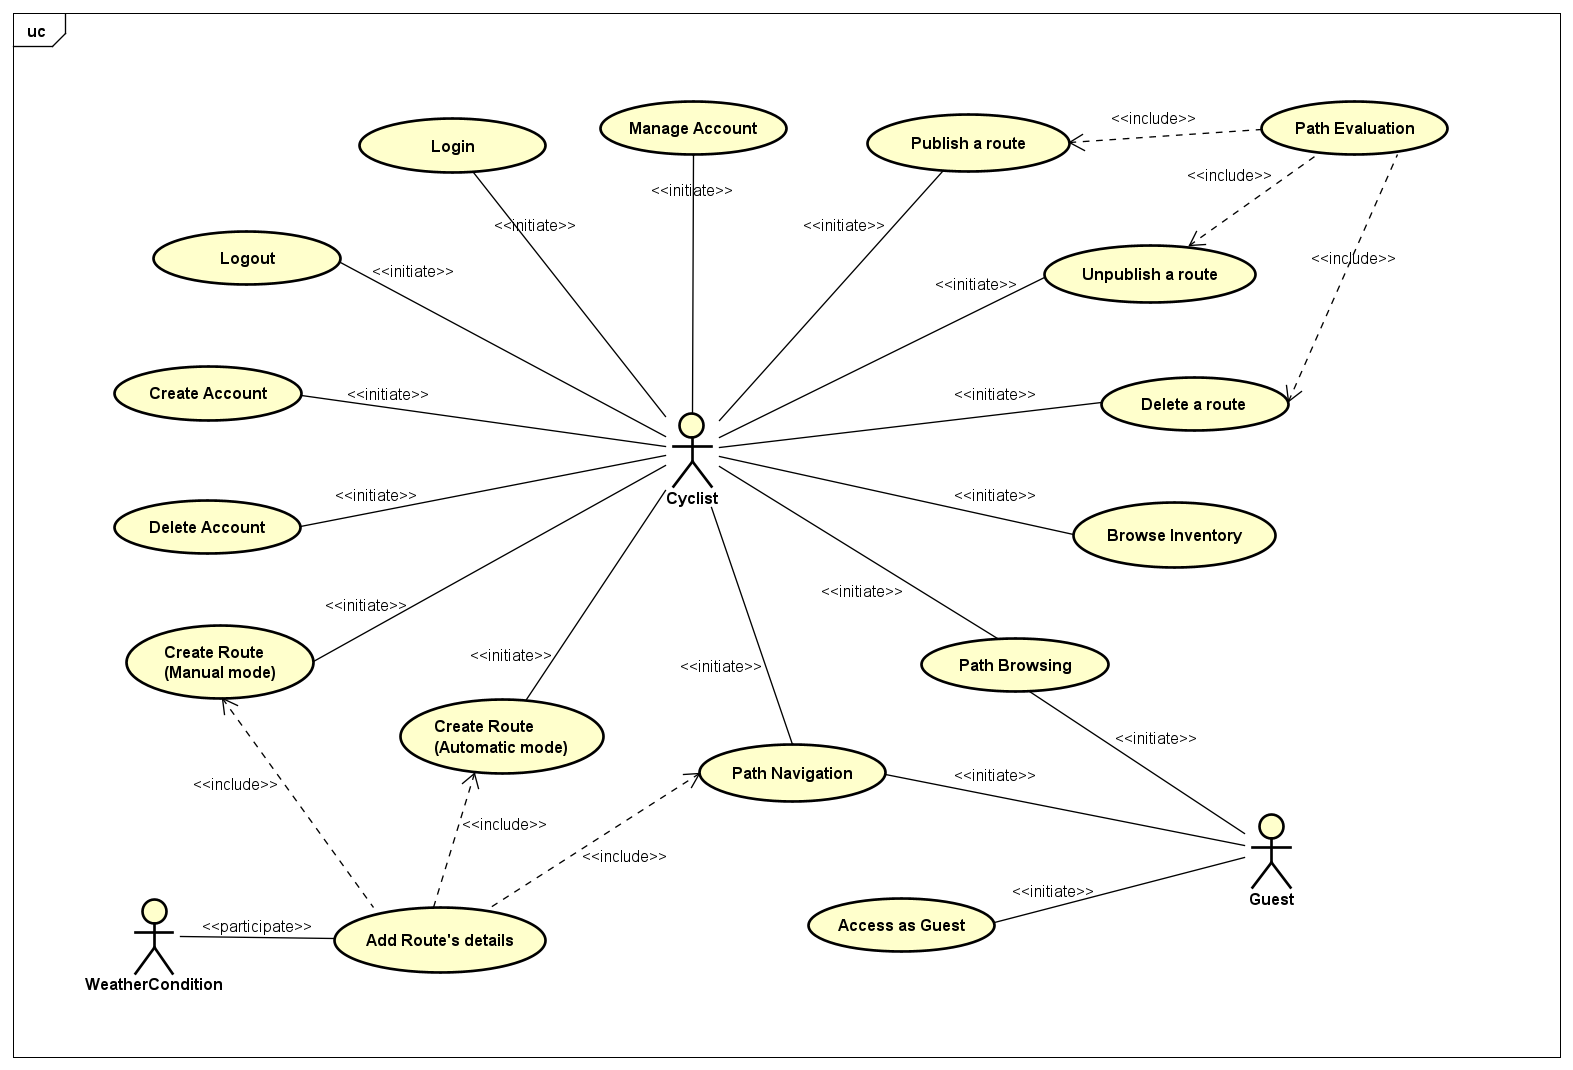
\includegraphics[width=\textwidth]{Images/UseCaseDiagram.png}
\caption{\label{fig:metamodel2}Use Case Diagram.}
\end{figure}
\newpage
\subsubsection{Use Cases}
\begin{itemize}
\item \textbf{UC1 - Create Account}\par\smallskip
\noindent
\begin{tabular}{|p{7cm}|p{7cm}|}
\hline
Name            & Create Account \\ \hline
Actors          & Cyclist\\ \hline
Entry Condition &  The Cyclist has not an account yet and they are on the \hyperref[fig:LoginSignUp]{authentication page}\\  \hline
Event Flow      &
\begin{enumerate}
    \item The Cyclist presses the button \textit{Sign Up}
    \item The system shows a registration form
    \item The Cyclist compiles the form providing his name, e-mail and password
    \item The Cyclist presses the button \textit{Sign Up}
    \item The system checks if the email has not already been used
\end{enumerate}
\\ \hline
Exit Condition  & The Cyclist has successfully registered to the platform and the system shows the \hyperref[fig:Homepage]{Homepage} \\ \hline
Exception       &  There already exist a cyclist with those e-mail; the system return to the entry condition showing an error message \textit{Cyclist already registered}\\ \hline
\end{tabular}
\bigskip
\item \textbf{UC2 - Login}\par\smallskip
\noindent
\begin{tabular}{|p{7cm}|p{7cm}|}
\hline
Name            & Login \\ \hline
Actors          & Cyclist \\ \hline
Entry Condition & The Cyclist has already created an account and he's on the \hyperref[fig:LoginSignUp]{authentication page} \\ \hline
Event Flow      &
\begin{enumerate}
    \item The Cyclist presses the \textit{Login} button
    \item The system shows the login form
    \item The Cyclist compiles the form inserting e-mail and password
    \item The Cyclist presses the \textit{Login} button
    \item The system checks if the credentials are correct
\end{enumerate}
\\ \hline
Exit Condition  & The Cyclist has successfully logged to the platform and the system shows the \hyperref[fig:Homepage]{Homepage}\\ \hline
Exception       & The credentials are not correct so the system shows an error message and shows again the [fig:LoginSignUp]{authentication page}
\\ \hline
\end{tabular}
\newpage
\item \textbf{UC3 - Guest Access}\par\smallskip
\noindent
\begin{tabular}{|p{7cm}|p{7cm}|}
\hline
Name            & Guest Access \\ \hline
Actors          & Guest \\ \hline
Entry Condition & The guest is on the \hyperref[fig:LoginSignUp]{authentication page}\\ \hline
Event Flow      &  
\begin{enumerate}
    \item The Guest presses the \textit{Continue as Guest} button
    \item The system shows an overlay with a message 'Continuing as a Guest, you can access only to limited features. Are you sure?'
    \item The Guest presses the confirm button \textit{Continue as Guest} on the overlay
\end{enumerate}
\\ \hline
Exit Condition  & The system shows the  \hyperref[fig:Homepage]{ Guest Homepage} (the other screens are locked)\\ \hline
Exception   & The Guest presses the \textit{Cancel} button and the system closes the overlay \\ \hline
\end{tabular}
\bigskip
\item \textbf{UC4 - Logout}\par\smallskip
\noindent
\begin{tabular}{|p{7cm}|p{7cm}|}
\hline
Name            & Logout \\ \hline
Actors          & Cyclist \\ \hline
Entry Condition & The Cyclist is logged into the system \\ \hline
Event Flow      & 
\begin{enumerate}
    \item The Cyclist presses the \textit{Account} button
    \item The system shows the account page 
    \item The Cyclist presses the \textit{Logout} button on the top of the page
    \item The system shows an overlay with a message 'Do you want to logout?'
    \item The Cyclist presses the confirm button \textit{Logout} on the overlay
\end{enumerate}
\\ \hline
Exit Condition  & The \hyperref[fig:LoginSignUp]{ authentication page} is shown \\ \hline
Exception      & The Cyclist presses the \textit{Cancel} button and the system closes the overlay \\ \hline
\end{tabular}
\newpage
\item \textbf{UC5 - Manage Account}\par\smallskip
\noindent
\begin{tabular}{|p{7cm}|p{7cm}|}
\hline
Name            & Manage Account \\ \hline
Actors          & Cyclist \\ \hline
Entry Condition & The Cyclist is logged into the system \\ \hline
Event Flow      &
\begin{enumerate}
    \item The Cyclist presses the \textit{Account} button
     \item The system shows the account page
    \item The Cyclist presses the  \textit{Edit Account} button
    \item The system shows a form where the Cyclist can edit his credentials, his account photo and his username
    \item The Cyclist edit his information and presses the  \textit{Confirm} button
\end{enumerate}
\\ \hline
Exit Condition  & The system shows the \hyperref[fig:Account]{Account Page}  with updated information \\ \hline
Exception       & The Cyclist inserts invalid data and the system shows an error message without updating the account
\\ \hline
\end{tabular}
\bigskip
\item \textbf{UC6 - Delete Account}\par\smallskip
\noindent
\begin{tabular}{|p{7cm}|p{7cm}|}
\hline
Name            & Delete  Account \\ \hline
Actors          & Cyclist \\ \hline
Entry Condition & The Cyclist is logged into the system \\ \hline
Event Flow      &
\begin{enumerate}
    \item The Cyclist presses the \textit{Account button}
    \item The system shows the Account page
    \item The Cyclist presses the  \textit{Delete Account} button on the bottom of the page
    \item The system shows an overlay with a message "Are you sure do you want to delete your account?"
    \item The Cyclist presses the confirm button \textit{Delete Account} on the overlay
\end{enumerate}
\\ \hline
Exit Condition  & The Cyclist is logged out from the platform, the system shows the  \hyperref[fig:LoginSignUp]{authentication page} and delete all the information related to the Cyclist \\ \hline
Exception       & The Cyclist presses the \textit{Cancel} button and the system closes the overlay
\\ \hline
\end{tabular}
\newpage
\item \textbf{UC7 - Create Route (Manual mode)}\par\smallskip
\noindent
\begin{tabular}{|p{7cm}|p{7cm}|}
\hline
Name            & Create Route (Manual mode) \\ \hline
Actors          & Cyclist \\ \hline
Entry Condition & The Cyclist is logged into the system \\ \hline
Event Flow      &
\begin{enumerate}
    \item The Cyclist presses the \textit{Create} button
    \item The system shows a page where the Cyclist has to choose the creation mode of the route
    \item The Cyclist presses on \textit{Start} button to manually create a route
    \item The system shows the manual creation page composed by a dynamic map that connects the Start Point, the Way Points and the End Point inserted by the Cyclist
    \item The Cyclist fills all the geographical point
    \item The Cyclist presses the \textbf{→} button to continue
\end{enumerate}
\\ \hline
Exit Condition  & The system shows the page to add route’s details and executes \textbf{UC9 - Add Route’s details} \\ \hline
Exception       & The Cyclist presses \textit{Back} button to go back and change the creation mode
\\ \hline
\end{tabular}
\newpage
\item \textbf{UC8 - Create Route (Automatic mode)}\par\smallskip
\noindent
\begin{tabular}{|p{7cm}|p{7cm}|}
\hline
Name            & Create Route (Automatic mode) \\ \hline
Actors          & Cyclist \\ \hline
Entry Condition & The Cyclist is logged into the system \\ \hline
Event Flow      &
\begin{enumerate}
    \item The Cyclist presses the \textit{Create} button
    \item The system shows a page where the Cyclist has to choose the creation mode of the route
    \item The Cyclist presses on \textit{Start tracking} button to start the automatically recording
    \item The system shows the automatic creation page composed with a button to effectively start the tracking when the Cyclist is ready
    \item The Cyclist presses the \textit{Start tracking} button to start the recording
    \item The system uses the device's sensors such as GPS, accelerometer and gyroscope to detect all the movements of the cyclist in order to obtain the set of streets and its status
    \item The Cyclist presses the \textit{Stop tracking} button to conclude the recording
    \item The system shows a page with a map to check the set of streets allowing the Cyclist to edit and confirm
    \item The Cyclist revises any errors and presses the confirm button
\end{enumerate}
\\ \hline
Exit Condition  & The system shows the  \hyperref[fig:CreateRouteManualDetails]{ page to add route’s details}  and executes \textbf{UC9 - Add Route’s details} \\ \hline
Exception       & The Cyclist presses \textit{Back} button to go back and change the creation mode
\\ \hline
\end{tabular}
\newpage
\item \textbf{UC9 - Add Route's details}\par\smallskip
\noindent
\begin{tabular}{|p{7cm}|p{7cm}|}
\hline
Name            & Add Route's details \\ \hline
Actors          & Cyclist, WeatherCondition \\ \hline
Entry Condition & The system shows the  \hyperref[fig:CreateRouteManualDetails]{ page to add route’s details} with precompiled and editable forms such as \textit{Start Point}, \textit{End Point}, \textit{Duration} and \textit{Distance} and other parameters to be filled \\ \hline
Event Flow      &
\begin{enumerate}
    \item The Cyclist provides missing information regarding the details of the route, adding the \textit{Description} through the forms and eventually edits the other precompiled forms
    \item The Cyclist evaluates the status of the route through the slider (deciding among bad, require maintenance, sufficient, medium, optimal)
    \item The Cyclist presses the \textit{Save} button

    \item The system asks for the weather condition in the date of the route 
    \item The WeatherCondition provides these information
    \item The system enriches the route's details with data provided by  WeatherCondition

    \item The system checks for the existence of another path with a set of streets compatible with the set of streets collected during route creation 
    \item If it does not exist, the system creates a new path for the current route
    \item The system adds the new route to the related path
    \item The system updates the account statistics, such as number of routes, total distance and total time.
\end{enumerate}
\\ \hline
Exit Condition  & The system saves the route into the related path and shows the  \hyperref[fig:Inventory]{path's details page} \\ \hline
Exception       &
\\ \hline
\end{tabular}
\newpage
\item \textbf{UC10 - Browse inventory}\par\smallskip
\noindent
\begin{tabular}{|p{7cm}|p{7cm}|}
\hline
Name            & Browse inventory \\ \hline
Actors          & Cyclist \\ \hline
Entry Condition & The Cyclist is logged into the system  \\ \hline
Event Flow      &
\begin{enumerate}
    \item The Cyclist presses the \textit{Inventory} button
    \item The system shows the Cyclist's inventory with the options to filter the paths displayed by status or by public paths and the options to sort the paths by date, distance and score
    \item The Cyclist presses on the path he wants to visualize
\end{enumerate}
\\ \hline
Exit Condition  & The system shows the \hyperref[fig:Inventory]{ path's details page} where the user can visualizes the map, the statistics (such as average time, distance, status and score), the list of his routes related to that path and a button to start navigation \\ \hline
Exception       &
\\ \hline
\end{tabular}
\bigskip
\item \textbf{UC11 - Path Browsing}\par\smallskip
\noindent
\begin{tabular}{|p{7cm}|p{7cm}|}
\hline
Name            & Path Browsing \\ \hline
Actors          & Cyclist, Guest \\ \hline
Entry Condition & The User is on the \hyperref[fig:Homepage]{Homepage} where he can visualize the parameters to perform the search and a list of top rated paths \\ \hline
Event Flow      &
\begin{enumerate}
    \item The User inserts a \textit{Start Point} and an \textit{End Point} in the dedicated forms, chooses a \textit{Tolerance} through the slider and then presses the \textit{Search Paths} button
    \item The system searches the paths that best fits the criteria and shows them ordered by \textit{Score}
    \item The User presses a path to select it
\end{enumerate}
\\ \hline
Exit Condition  & The system shows the p\hyperref[fig:Inventory]{ path's details page} \\ \hline
Exception       & User go back and changes the selected path
\\ \hline
\end{tabular}
\newpage
\item \textbf{UC12 - Path Navigation}\par\smallskip
\noindent
\begin{tabular}{|p{7cm}|p{7cm}|}
\hline
Name            & Path Navigation \\ \hline
Actors          & Cyclist, Guest \\ \hline
Entry Condition & The User is on the \hyperref[fig:Inventory]{path's details page} \\ \hline
Event Flow      & 
\begin{enumerate}
    \item The User presses the \textit{Start Navigation} button
    \item The system shows the navigation page with a map to guide the User along the path in real time
    \item As soon as the User reaches the end point, the system stops the navigation and shows a message "Path completed"
    \item The User presses the \textit{Continue} button
\end{enumerate}
\\ \hline
Exit Condition  & The User is a Cyclist and the system shows the page to add route's details and executes \textbf{UC9-Add Route’s details } \\ \hline
Exception       & The User is a Guest and the system shows a message "You have to login to save a route" and a button to perform authentication
\\ \hline
\end{tabular}
\newpage
\item \textbf{UC13 - Publish a route}\par\smallskip
\noindent
\begin{tabular}{|p{7cm}|p{7cm}|}
\hline
Name            & Publish a route \\ \hline
Actors          & Cyclist \\ \hline
Entry Condition & Cyclist is in the \hyperref[fig:Inventory]{ inventory} and the route is private\\ \hline
Event Flow      &
\begin{enumerate}
    \item The Cyclist expands the view of the route that he wants to publish  
    \item The system shows the button to publish or delete the route 
    \item The Cyclist presses the \textit{Publish} button
    \item The system shows an overlay with the message \textit{"All the information about this route will be visible to other users. Do you want to continue?"} 
    \item The Cyclist presses the \textit{Continue} button on the overlay
    \item The system executes \textbf{UC15 - Path Evaluation} considering the route to be published and eventually also the others already published
    \item If the path is not already public, the system makes it public
    \item The system makes the route public and now it is visible by other users inside the related path.
    \item The system updates the number of published routes in the account statistics.
\end{enumerate}
\\ \hline
Exit Condition  &  The system shows the \textit{Unpublish} button\\ \hline
Exception       &
\\ \hline
\end{tabular}
\newpage
\item \textbf{UC14 - Unpublish a route}\par\smallskip
\noindent
\begin{tabular}{|p{7cm}|p{7cm}|}
\hline
Name            & Unpublish a route \\ \hline
Actors          & Cyclist \\ \hline
Entry Condition & Cyclist is in the \hyperref[fig:Inventory]{ inventory} and the route is public\\ \hline
Event Flow      &
\begin{enumerate}
    \item The Cyclist expands the view of the route that he wants to unpublish  
    \item The system shows the button to unpublish or delete the route 
    \item The Cyclist presses the \textit{Unpublish} button
    \item The system shows an overlay with the message \textit{"All the information about this route will be no more visible to other users. Do you want to continue?"} 
    \item The Cyclist presses the \textit{Continue} button on the overlay
    \item The system checks the existence of at least another public route for that path
    \item If there is, the system executes \textbf{UC15 - Path Evaluation}, excluding the route to be unpublished
    \item Else the system makes the path not public until another route will be published again
    \item The system makes the route private and now it is visible only in the inventory
    \item The system updates the number of published routes in the account statistics.
\end{enumerate}
\\ \hline
Exit Condition  & The system shows the \textit{Publish} button \\ \hline
Exception       &
\\ \hline
\end{tabular}
\newpage
\item \textbf{UC15 - Path Evaluation}\par\smallskip
\noindent
\begin{tabular}{|p{7cm}|p{7cm}|}
\hline
Name            & Path Evaluation \\ \hline
Actors          & Cyclist \\ \hline
Entry Condition & The system has to update the status and the score of a path \\ \hline
Event Flow      & \begin{enumerate}
    \item The system gets all the public routes having the most recent date available in the path to be updated 
    \item If there is only one route, the system updates the path status with the status of that route
    \item Else, the system updates the path status with the value corresponding to the status shared by the largest number of routes (in case of a tie, the system computes the average by treating the status values as numerical values from 1 to 5)
    \item After the status computation, the system updates the other path's statistics, such as the average time and distance
    \item The system calculates and updates the path's score based on path's status and average speed
\end{enumerate}
\\ \hline
Exit Condition  & The system has updated the status and the score of a path\\ \hline
Exception       &
\\ \hline
\end{tabular}
\newpage
\item \textbf{UC16 - Delete a route}\par\smallskip
\noindent
\begin{tabular}{|p{7cm}|p{7cm}|}
\hline
Name            & Delete a route \\ \hline
Actors          & Cyclist \\ \hline
Entry Condition &  Cyclist is in the \hyperref[fig:Inventory]{inventory}\\ \hline
Event Flow      &
\begin{enumerate}[label=\arabic*.]
    \item The Cyclist expands the view of the route that he wants to delete  
    \item The system shows the button to publish/unpublish or delete the route 
    \item The Cyclist presses the \textit{Delete} button
    \item The system shows an overlay with the message \textit{"All the information about this route will be deleted forever. Do you want to continue?"} 
    \item The Cyclist presses the \textit{Continue} button on the overlay 
    \item The system retrieves the other private and public routes of the path related to the current route
    \item If the route is the last one of that path, the system deletes the path
    \item Else if the route is published 
        \begin{enumerate} [label=\arabic{enumi}.\arabic*.]
            \item If there are other published routes, the system executes \textbf{UC15 - Path Evaluation}
            \item Else the system makes the path private 
        \end{enumerate} 
    \item The system deletes the route
    \item The system updates the account statistics, such as number of routes, number of published routes, total distance and total time.
\end{enumerate}
\\ \hline
Exit Condition  & The system shows the updated inventory page \\ \hline
Exception       &
\\ \hline
\end{tabular}
\end{itemize}
\newpage
\subsubsection{Sequence Diagrams}
\begin{itemize}
\item \textbf{SD1 - Create Account}\par\smallskip
\noindent
\begin{figure}[H]
\centering

\includegraphics[width=\textwidth]{Images/SD/SD1_CreateAccount.png}
\caption{\label{fig:metamodel2}Sequence Diagram related to UC1 - Create Account}
\end{figure}
\newpage
\item \textbf{SD2 - Login}\par\smallskip
\noindent
\begin{figure}[H]
\centering

\includegraphics[width=\textwidth]{Images/SD/SD2_Login.png}
\caption{\label{fig:metamodel2}Sequence Diagram related to UC2 - Login}
\end{figure}
\newpage
\item \textbf{SD3 - Guest Access}\par\smallskip
\noindent
\begin{figure}[H]
\centering

\includegraphics[width=0.9\textwidth]{Images/SD/SD3_GuestAccess.png}
\caption{\label{fig:metamodel2}Sequence Diagram related to UC3 - Guest Access}
\end{figure}
\newpage
\item \textbf{SD4 - Logout}\par\smallskip
\noindent
\begin{figure}[H]
\centering

\includegraphics[width=0.9\textwidth]{Images/SD/SD4_Logout.png}
\caption{\label{fig:metamodel2}Sequence Diagram related to UC4 - Logout}
\end{figure}
\newpage
\item \textbf{SD5 - Manage Account}\par\smallskip
\noindent
\begin{figure}[H]
\centering
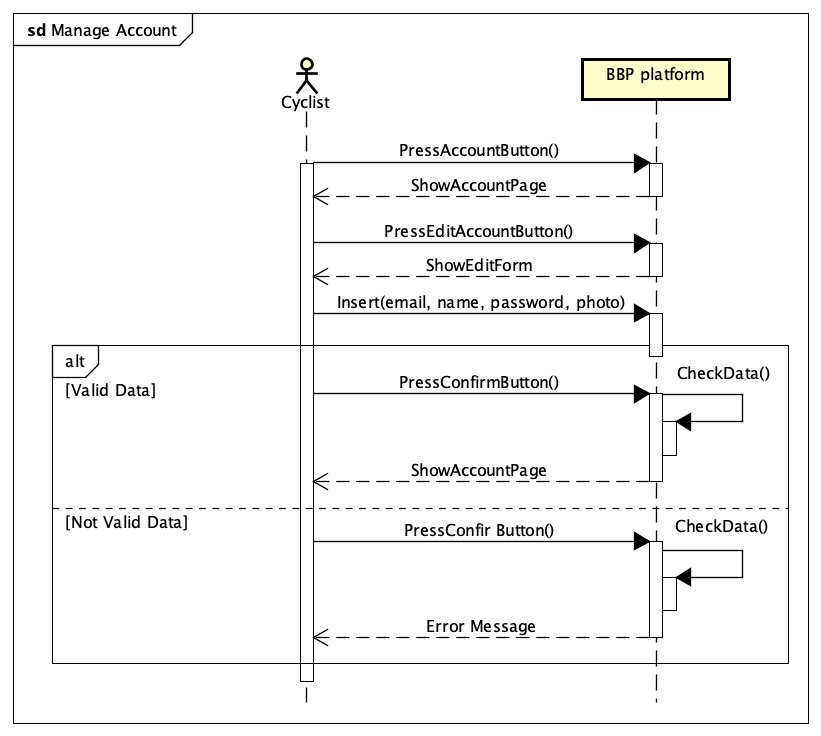
\includegraphics[width=\textwidth]{Images/SD/SD5_Manage Account.png}
\caption{\label{fig:metamodel2}Sequence Diagram related to UC5 - Manage Account}
\end{figure}
\newpage
\item \textbf{SD6 - Delete Account}\par\smallskip
\noindent
\begin{figure}[H]
\centering

\includegraphics[width=\textwidth]{Images/SD/SD6_DeleteAccount.png}
\caption{\label{fig:metamodel2}Sequence Diagram related to UC6 - Delete Account}
\end{figure}
\newpage
\item \textbf{SD7 - Create Route (Manual Mode)}\par\smallskip
\noindent
\begin{figure}[H]
\centering
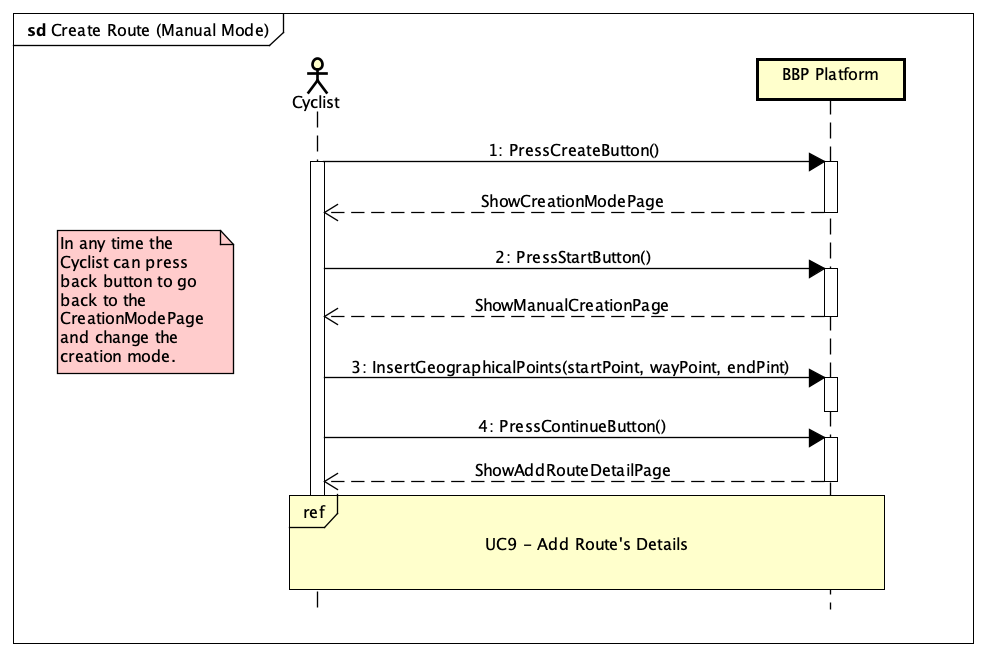
\includegraphics[width=\textwidth]{Images/SD/SD7_CreateRouteMM .png}
\caption{\label{fig:metamodel2}Sequence Diagram related to UC7 - Create Route (Manual Mode)}
\end{figure}
\newpage
\item \textbf{SD8 - Create Route (Automatic Mode)}\par\smallskip
\noindent
\begin{figure}[H]
\centering

\includegraphics[width=\textwidth]{Images/SD/SD8_CreateRouteAM.png}
\caption{\label{fig:metamodel2}Sequence Diagram related to UC8 - Create Route (Automatic Mode)}
\end{figure}
\newpage
\item \textbf{SD9 - Add Route's Details}\par\smallskip
\noindent
\begin{figure}[H]
\centering

\includegraphics[width=\textwidth]{Images/SD/SD9_AddRoute'sDetails.png}
\caption{\label{fig:metamodel2}Sequence Diagram related to UC9 - Add Route's Details}
\end{figure}
\newpage
\item \textbf{SD10 - Browse Inventory}\par\smallskip
\noindent
\begin{figure}[H]
\centering

\includegraphics[width=1\linewidth]{Images/SD/SD10_BrowseInventory.png}
\caption{\label{fig:metamodel2}Sequence Diagram related to UC10 - Browse Inventory}
\end{figure}
\bigskip
\item \textbf{SD11 - Path Browsing}\par\smallskip
\noindent
\begin{figure}[H]
\centering

\includegraphics[width=1\linewidth]{Images/SD/SD11_PathBrowsing.png}
\caption{\label{fig:metamodel2}Sequence Diagram related to UC11 - Path Browsing}
\end{figure}
\newpage
\item \textbf{SD12 - Path Navigation}\par\smallskip
\noindent
\begin{figure}[H]
\centering

\includegraphics[width=\textwidth]{Images/SD/SD12_PathNavigation.png}
\caption{\label{fig:metamodel2}Sequence Diagram related to UC12 - Path Navigation}
\end{figure}
\newpage
\item \textbf{SD13 - Publish a route}\par\smallskip
\noindent
\begin{figure}[H]
\centering

\includegraphics[width=\textwidth]{Images/SD/SD13_PublishARoute.png}
\caption{\label{fig:metamodel2}Sequence Diagram related to UC13 - Publish a route}
\end{figure}
\newpage
\item \textbf{SD14 - Unpublish a route}\par\smallskip
\noindent
\begin{figure}[H]
\centering

\includegraphics[width=\textwidth]{Images/SD/SD14_UnpublishARoute.png}
\caption{\label{fig:metamodel2}Sequence Diagram related to UC14 - Unpublish a route}
\end{figure}
\newpage
\item \textbf{SD15 - Path Evaluation}\par\smallskip
\noindent
\begin{figure}[H]
\centering

\includegraphics[width=\textwidth]{Images/SD/SD15_PathEvaluation.png}
\caption{\label{fig:metamodel2}Sequence Diagram related to UC15 - Path Evaluation}
\end{figure}
\newpage
\item \textbf{SD16 - Delete a route}\par\smallskip
\noindent
\begin{figure}[H]
\centering

\includegraphics[width=\textwidth]{Images/SD/SD16_DeleteARoute.png}
\caption{\label{fig:metamodel2}Sequence Diagram related to UC16 - Delete a route}
\end{figure}
\end{itemize}
\newpage
\subsubsection{Activity Diagram}
\begin{itemize}
\item \textbf{AD16 - Delete a route} 
\noindent
\begin{figure}[H]
\centering
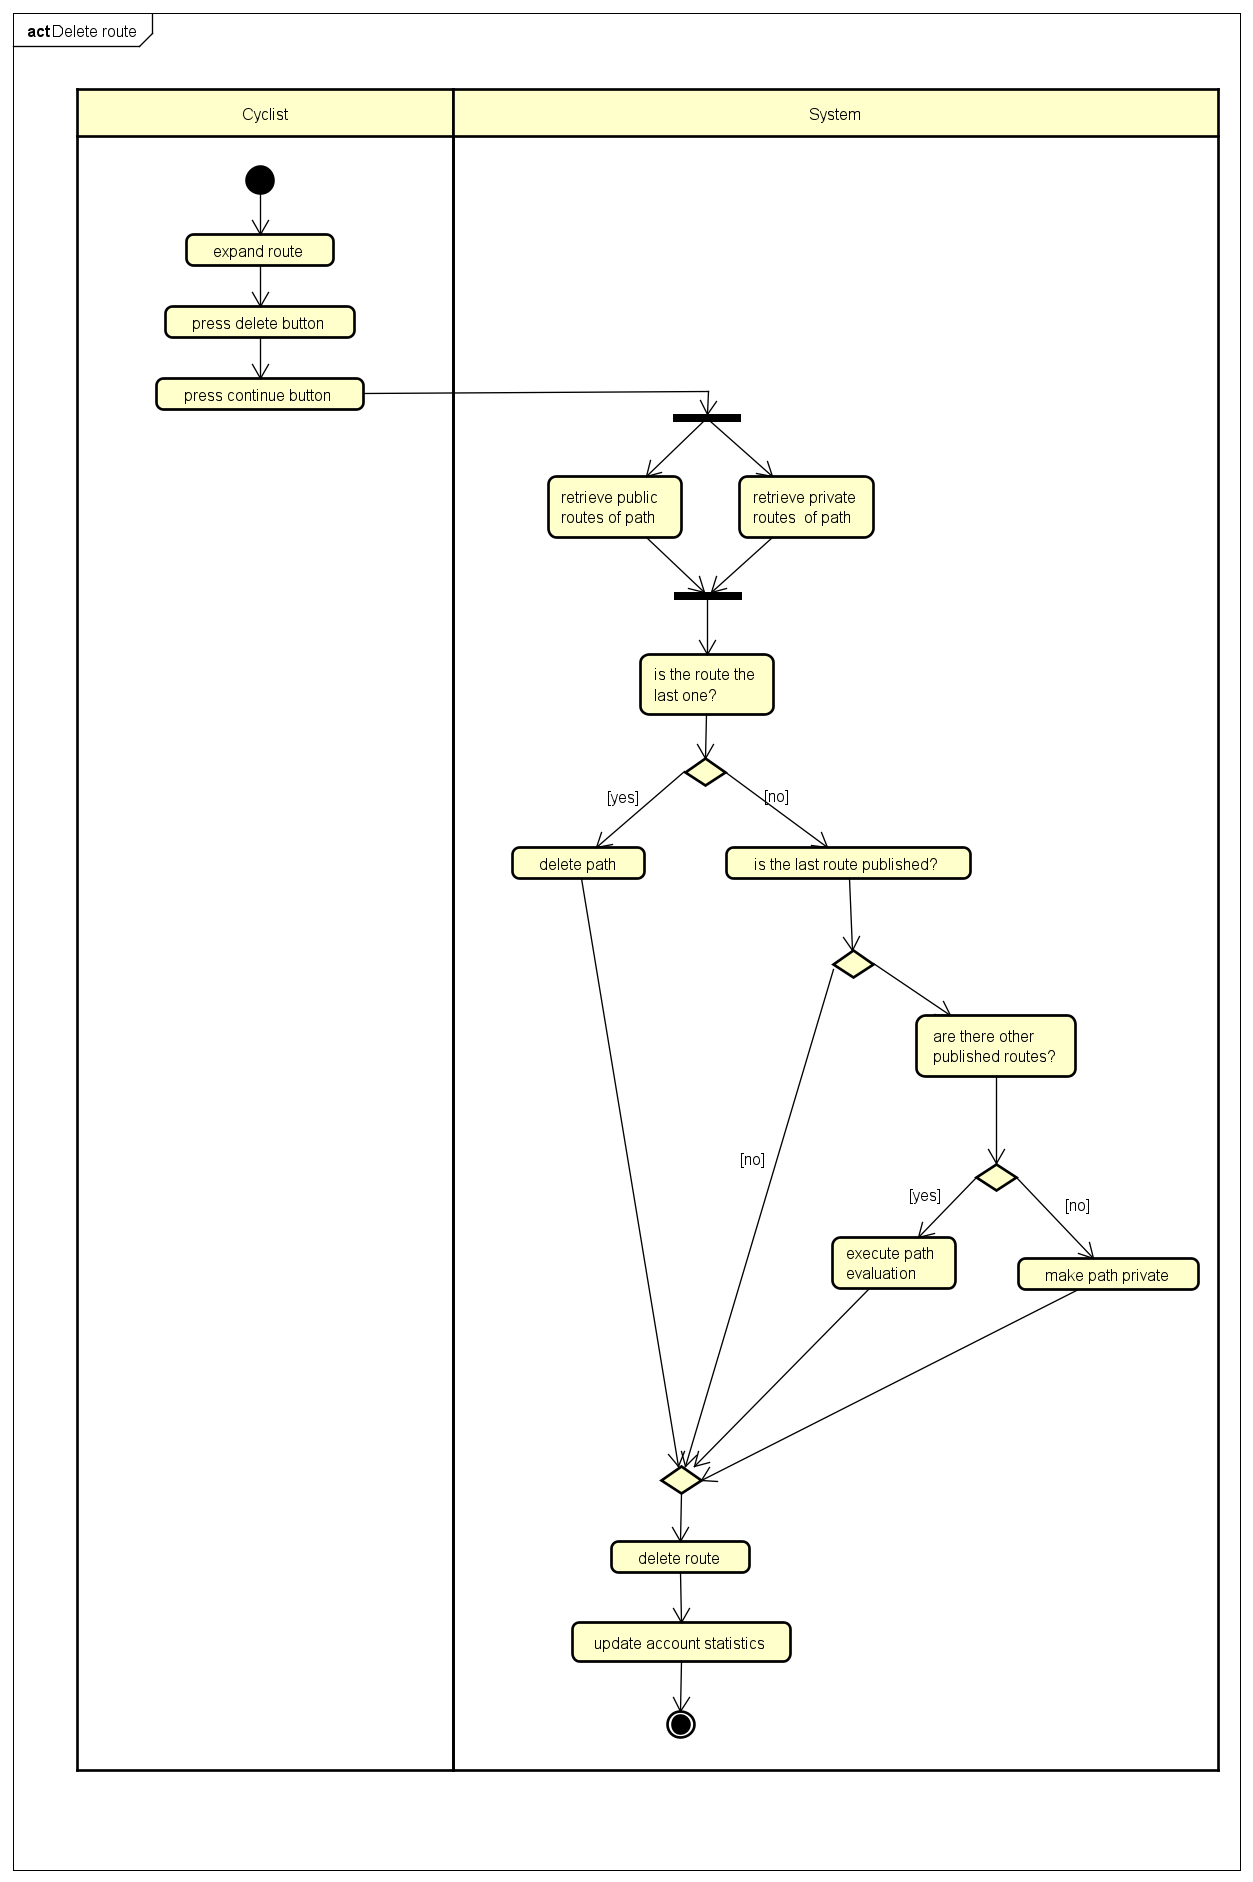
\includegraphics[width=0.8\linewidth]{Images/AD/AD16_DeleteARoute.png}
\caption{\label{fig:metamodel2}Activity Diagram related to UC16 - Delete a route}
\end{figure}
\end{itemize}
The activity diagram in the figure is intended to clarify the flow of actions of the use case \textbf{UC16 - Delete a route}. Since the operation is complex, two complementary representations are provided to allow its analysis from different perspectives.
\subsubsection{Requirement Mapping}
\begin{table}[h!]
\centering
\begin{tabular}{|p{7cm}|p{7cm}|}
\hline
\multicolumn{2}{|p{14cm}|}{\textbf{G1:} Cyclists can manually create bike routes or alternatively be assisted by the system to automatically track the paths thanks to the mobile device's sensors. Subsequently, the paths can be reviewed and enriched with general information and with a status before being saved inside the inventory.} \\ \hline
\textbf{R1:} The platform allows the Cyclists to create an account. &
\textbf{D1:} The cyclist’s account data is correct. \\ 
\textbf{R2:} The platform allows Cyclists to authenticate.& 
\textbf{D2:} The cyclist remembers his credentials.\\ 
\textbf{R4:} The platform allows Cyclists to view their personal account. & 
\textbf{D3:} The cyclist manually adds a path only after actually completing it.\\ 
\textbf{R5:} The platform allows Cyclists to modify their personal account. & 
\textbf{D4:} When creating and evaluating a route, the cyclist inputs accurate and realistic information.\\ 
\textbf{R6:} The platform allows the Cyclists to create a new route through a manual creation process. & 
\textbf{D5:} Reliable meteorological information.\\ 
\textbf{R7:} The platform allows the Cyclists to create a new route through an automatic creation process. & 
\textbf{D6:} If cyclists use GPS, accelerometer and gyroscope we assume that they are accurate and work correctly\\ 
\textbf{R8:} The platform allows the Cyclists to confirm and complete the automatically acquired information.& 
\textbf{D9:} All users have a reliable internet connection.
\\
\textbf{R9:} The platform collects data from the device sensors.&\\
\textbf{R10:} The platform collects weather data and enriches the path’s statistics.&\\
\textbf{R11:} The platform allows the Cyclists to evaluate the status of a route. &\\
\textbf{R15:} The platform allows the User to view the details of a path such as the map, the statistics and the status.&\\
\textbf{R16:} The platform allows the User to visualize the details of the routes related to a path.&\\
\hline
\end{tabular}
\end{table}
\newpage
\begin{table}[h!]
\centering
\begin{tabular}{|p{7cm}|p{7cm}|}
\hline
\multicolumn{2}{|p{14cm}|}{\textbf{G2:} Cyclists can visualize and manage their own inventory and search for their saved routes with their statistics, status and meteorological information provided by external services.} \\ \hline
\textbf{R1:} The platform allows the Cyclists to create an account. & 
\textbf{D1:} The cyclist’s account data is correct. \\ 
\textbf{R2:} The platform allows Cyclists to authenticate. & 
\textbf{D2:} The cyclist remembers his credentials.\\ 
\textbf{R4:} The platform allows Cyclists to view their personal account. &
\textbf{D5:} Reliable meteorological information.\\ 
\textbf{R5:} The platform allows Cyclists to modify their personal account. & \\ 
\textbf{R13:} The platform allows the Cyclists to delete a route. & 
\textbf{D9:} All users have a reliable internet connection.\\ 
\textbf{R14:} The platform allows the Cyclists to visualize a list of paths in the personal inventory with the possibility to filter them. & \\ 
\textbf{R15:} The platform allows the User to view the details of a path such as the map, the statistics and the status. &\\
\textbf{R16:} The platform allows the User to visualize the details of the routes related to a path. &\\
\hline
\end{tabular}
\end{table}
\begin{table}[h!]
\centering
\begin{tabular}{|p{7cm}|p{7cm}|}
\hline
\multicolumn{2}{|p{14cm}|}{\textbf{G3:} Cyclists can publish their routes, sharing them with the community, creating a social component in the system where users can discover different paths proposed by others.} \\ \hline
\textbf{R1:} The platform allows the Cyclists to create an account. & 
\textbf{D1:} The cyclist’s account data is correct. \\ 
\textbf{R2:} The platform allows Cyclists to authenticate.& 
\textbf{D2:} The cyclist remembers his credentials.\\
\textbf{R3:} The platform allows the access as a Guest. & 
\textbf{D9:} All users have a reliable internet connection.\\
\textbf{R4:}The platform allows Cyclists to view their personal account.& \\
\textbf{R5:} The platform allows Cyclists to modify their personal account.& \\
\textbf{R12:}The platform allows the Cyclists to publish/unpublish a route. &  \\
\textbf{R15:} The platform allows the User to view the details of a path such as the map, the statistics and the status. & \\
\textbf{R16:} The platform allows the User to visualize the details of the routes related to a path.& \\
\textbf{R20} The platform merges the status when more than one is present.&\\
\textbf{R21} The platform compu     tes a score for each path based on path's status and average speed.&\\
\hline
\end{tabular}
\end{table}
\newpage
\begin{table}[h!]
\centering
\begin{tabular}{|p{7cm}|p{7cm}|}
\hline
\multicolumn{2}{|p{14cm}|}{\textbf{G4:} Given a starting point and a destination, the software suggests the best paths to the user visualizing them in a ranking based on scores and allowing the user to be guided by a navigation system along the selected path.} \\ \hline
\textbf{R1:} The platform allows the Cyclists to create an account.& 
\textbf{D2:} The cyclist remembers his credentials. \\
\textbf{R2:} The platform allows Cyclists to authenticate.& 
\textbf{D4:} When creating and evaluating a route, the cyclist inputs accurate and realistic information.\\ 
\textbf{R3:} The platform allows the access as a Guest.& 
\textbf{D5:} Reliable meteorological information.\\ 
\textbf{R8:} The platform allows the Cyclists to confirm and complete the automatically acquired information.& 
\textbf{D6:} If cyclists use GPS, accelerometer and gyroscope we assume that they are accurate and work correctly\\ 
\textbf{R9:} The platform collects data from the device sensors.& 
\textbf{D7:} There are always paths available from point A to point B for any tollerance level.\\
\textbf{R10:} The platform collects weather data and enriches the path’s statistics.& 
\textbf{D8:} The starting and ending point are reasonable, so that they do not necessarily require the use of other
means of transportation.\\
\textbf{R11:} The platform allows the Cyclists to evaluate the status of a route. & 
\textbf{D9:} All users have a reliable internet connection. \\
\textbf{R15:} The platform allows the User to view the details of a path such as the map, the statistics and the status. &\\
\textbf{R16:} The platform allows the User to visualize the details of the routes related to a path.& \\
\textbf{R17:} The platform allows the User to search a path by setting the start and the end points with a kilometer tolerance.& \\
\textbf{R18:} The platform suggests to the User a list of available routes ranked by score. & \\
\textbf{R19:} bbp calcola il punteggio per ogni percorso (status/tempo impiegato) & \\
\textbf{R20:} The platform merges the status when more than one is present.& \\
\textbf{R21:} The platform computes a score for each path based on path's status and average speed.& \\
\hline
\end{tabular}
\end{table}
\clearpage
\subsection{Performance Requirements}
The system must guarantee adequate performance to ensure a smooth and responsive user experience under normal and peak usage conditions.\\[4pt]  
Core functionalities such as user authentication, route visualization, and path search must respond within few seconds. Automatic data acquisition from mobile sensors must be handled in near real-time, without causing significant delays or excessive battery consumption. The system must be able to support multiple concurrent users, scaling appropriately when there is an increasing number of active cyclists without degradation of service quality.
\subsection{Design Constraints}
\subsubsection{Standards compliance}
To conform the system with standards for data protection, the communication must use HTTPS protocol for secure data exchange. Moreover, the data management must adhere to applicable regulations (e.g., GDPR), ensuring protection of users’ personal data.
\subsubsection{Hardware limitations}
The platform is primarily intended for execution on mobile devices, which impose constraints in terms of processing power, memory, storage, and battery capacity.
The system must be designed to efficiently use hardware resources, avoiding intensive computations on the mobile devices whenever possible. Access to sensors such as GPS, accelerometer, and gyroscope depends on the availability and accuracy provided by the device hardware.
\subsubsection{Other constraints}
The system architecture must support interoperability with external services, whose availability and interfaces may impose additional constraints.
\subsection{Software System Attribute}
\subsubsection{Reliability}
The system must operate correctly and consistently under normal conditions, minimizing the occurrence of failures. In case of errors or unexpected conditions, the system must handle them rapidly, preventing data corruption and preserving system integrity.
\subsubsection{Availability}
The system must be available to users for at least 99\% of the time, especially during daylight hours and the scheduled maintenance should be planned in the night hours where the number of active users is expected to be lower. \\[4pt]  
Critical services, such as route creation or path search and navigation, must be designed to minimize downtime and ensure continuity of service without delay.
\subsubsection{Security}
The system must protect all exchanged and stored data from unauthorized access. Sensitive information, such as user credentials and real-time location data, must be transmitted using secure communication protocols and encrypted when necessary. \\[4pt]  
Authentication mechanism must be enforced to ensure that only authorized users can access restricted functionalities and to prevent cyber attacks, such as SQL injection.
\subsubsection{Maintainability}
The system must be well-documented and designed following modular principles to facilitate maintenance and future enhancements.
Changes to one component must have minimal impact on others, allowing easier bug fixing, updates, and future feature implementations.
\subsubsection{Portability}
The system must be portable across different mobile devices with different operative systems, requiring minimal adaptation of user interfaces. The platform is not intended to be used on desktop devices or in general devices that cannot be carried during a bike ride.